\documentclass[a4paper]{book}
\usepackage{makeidx}
\usepackage{graphicx}
\usepackage{multicol}
\usepackage{float}
\usepackage{listings}
\usepackage{color}
\usepackage{ifthen}
\usepackage[table]{xcolor}
\usepackage{textcomp}
\usepackage{alltt}
\usepackage{ifpdf}
\ifpdf
\usepackage[pdftex,
            pagebackref=true,
            colorlinks=true,
            linkcolor=blue,
            unicode
           ]{hyperref}
\else
\usepackage[ps2pdf,
            pagebackref=true,
            colorlinks=true,
            linkcolor=blue,
            unicode
           ]{hyperref}
\usepackage{pspicture}
\fi
\usepackage[utf8]{inputenc}
\usepackage{mathptmx}
\usepackage[scaled=.90]{helvet}
\usepackage{courier}
\usepackage{doxygen}
\lstset{language=C++,inputencoding=utf8,basicstyle=\footnotesize,breaklines=true,breakatwhitespace=true,tabsize=8,numbers=left }
\makeindex
\setcounter{tocdepth}{3}
\renewcommand{\footrulewidth}{0.4pt}
\begin{document}
\hypersetup{pageanchor=false}
\begin{titlepage}
\vspace*{7cm}
\begin{center}
{\Large JUMPDatabase \\[1ex]\large 1.0 }\\
\vspace*{1cm}
{\large Generated by Doxygen 1.7.3}\\
\vspace*{0.5cm}
{\small Tue Mar 8 2011 12:17:15}\\
\end{center}
\end{titlepage}
\clearemptydoublepage
\pagenumbering{roman}
\tableofcontents
\clearemptydoublepage
\pagenumbering{arabic}
\hypersetup{pageanchor=true}
\chapter{JUMP Database Programming Guide}
\label{index}\hypertarget{index}{}{\bfseries JUMP Database Module} is an collection of classes that are wrappers and facades around the \href{http://developer.apple.com/library/mac/#documentation/cocoa/conceptual/CoreData/cdProgrammingGuide.html}{\tt Apple Core Data Framework}.\par
 \par
 You should have at least an basic experiencie with this powerful Apple framework to fully understand this module, he doesn't abstract or replace the Core Data, it just make your life more easy.\par
 \par
 The main component of this module are the \hyperlink{interface_j_p_d_b_manager}{Database Manager}. The manager center the main Core Data components in a single class and facilitate a collection of methods to perform main tasks around it. Also the manager could be used as a \hyperlink{interface_j_p_d_b_manager_singleton}{Singleton Instance} facilitating even more your database operations.

This diagram shows all components of the Database Manager operations and his components.\par
 \par
 

\subsection*{Learn more about this module in the following sections:}


\begin{DoxyItemize}
\item \hyperlink{basic_uses}{Basic Uses}
\item \hyperlink{errors}{Handling Errors}
\item \hyperlink{queries}{Performing Queries} 
\end{DoxyItemize}
\chapter{Handling Errors}
\label{errors}
\hypertarget{errors}{}
There are two types of errors that the \hyperlink{interface_j_p_d_b_manager}{Database Manager} let you known.\hypertarget{errors_fatal_errors}{}\section{Fatal Errors or Exceptions}\label{errors_fatal_errors}
This is are errors that will prevent the {\bfseries Database Manager} or your application to work correctly. On most part of cases you're trying to retrieve some data that doesn't exist or something like that. So an exception ({\bfseries NSException}) is raised and if isn't catched will interrupt your application. You always can use an {\bfseries try..catch} block to avoid that.

This is are the exceptions raised by the Manager. This exceptions are defined on \hyperlink{_j_p_d_b_manager_definitions_8h_source}{JPDBManagerDefinitions.h} file.\hypertarget{errors_JPDBManagerActionException}{}\subsection{JPDBManagerActionException}\label{errors_JPDBManagerActionException}
This kind of exception is raised when is impossible to perform an \hyperlink{interface_j_p_d_b_manager_action}{Database Action}.\hypertarget{errors_JPDBManagerStartException}{}\subsection{JPDBManagerStartException}\label{errors_JPDBManagerStartException}
This kind of exception is raised when is impossible to start the {\bfseries Core Data} environment.\hypertarget{errors_JPDBInvalidInitiator}{}\subsection{JPDBInvalidInitiator}\label{errors_JPDBInvalidInitiator}
This kind of exception is raised when you try to use some 'init' method that is protected. From an Abstract or an Singleton Class for example.\hypertarget{errors_errors_section}{}\section{Errors}\label{errors_errors_section}
This is are errors that doesn't prevent the {\bfseries Database Manager} or your application to work correctly. If you doesn't handle this errors they will be logged to the console, nothing else.

To handle this errors you should sign to the {\bfseries NSNotificationCenter} with the {\bfseries JPDBManagerErrorNotification} Key to receive detailed information. This Key is defined in \hyperlink{_j_p_d_b_manager_definitions_8h_source}{JPDBManagerDefinitions.h} file.\par
 \par
 The {\bfseries Database Manager} post an {\bfseries NSNotification} when some error ocurr performing one operation. \par
 \par
 The {\bfseries NSNotification} object encapsulate an {\bfseries NSError} with the cause and description. You can retrieve the manager that generates the error acessing the {\bfseries JPDBManagerErrorNotification} Key on the {\bfseries userInfo} dictionary. 
\chapter{Performing Queries}
\label{queries}
\hypertarget{queries}{}
The {\bfseries Database Manager} post an {\bfseries NSNotification} when some error ocurr performing one operation. Sign to the {\bfseries NSNotificationCenter} with the {\bfseries JPDBManagerErrorNotification} Key to receive detailed information.\par
 \par
 The {\bfseries NSNotification} object encapsulate an {\bfseries NSError} with the cause and descrption. You can retrieve the manager that generates he error acessing the {\bfseries JPDBManagerErrorNotification} Key on the {\bfseries userInfo} dictionary. 
\chapter{Basic Uses}
\label{basic_uses}
\hypertarget{basic_uses}{}
This page show some basic examples of usage for the {\bfseries JUMP Database Module}.\par
 \par
 On our examples we presume that you have your Core Data models created. See \href{http://developer.apple.com/library/mac/#documentation/cocoa/conceptual/CoreData/cdProgrammingGuide.html}{\tt Introduction to Core Data Programming Guide} \par
 to learn more about it.\par
 \par
\hypertarget{basic_uses_init_manager}{}\section{Initializing the Database Manager}\label{basic_uses_init_manager}
The first step to start to work with the \hyperlink{interface_j_p_d_b_manager}{Database Manager} is initialize the all system. 
\begin{DoxyCode}
 [[JPDBManagerSingleton sharedInstance] startCoreData];
\end{DoxyCode}
 The above code perform a lot of tasks. He initiate the full Core Data model and create the persistent stores if needed. We're using an {\bfseries Singleton Instance} of the Manager. You always can initiate one regular instance, but in the most common cases you will use this way.\hypertarget{basic_uses_db_action}{}\section{Performing Database Actions}\label{basic_uses_db_action}
Database operations isn't called directy to the manager. Instead we create one instance of the \hyperlink{interface_j_p_d_b_manager_action}{JPDBManagerAction} class, configure the data and settings to perform some \href{http://en.wikipedia.org/wiki/Create,_read,_update_and_delete}{\tt CRUD} operation and finally run this action. Yes, looks like a lot of work, but actually is not. Let's see some examples: 
\begin{DoxyCode}
 id newRecord = [JPDatabaseManager createNewRecordForEntity:@"MyEntity"];
\end{DoxyCode}
 This is was really simple, isn't? Let's see this same operation on a more custom fashion: 
\begin{DoxyCode}
 JPDBManagerAction *anAction = [[JPDBManagerSingleton sharedInstance] 
      getDatabaseAction];
 [anAction setCommitTransaction:YES];
 id newRecord = [anAction createNewRecordForEntity:@"MyEntity"];
\end{DoxyCode}
 Well this looks a litle bit more complicated. Let's understand this two processes: The first one uses the {\bfseries JPDatabaseManager} convenient macro shortcut that returns an \hyperlink{interface_j_p_d_b_manager_action}{JPDBManagerAction} instance and perform this method in only one pass, is pure convenience. This macro is declared in the \hyperlink{_j_p_d_b_manager_definitions_8h_source}{JPDBManagerDefinitions.h} file. \par
 \par
 The second way needs more steps, but you should use that way when you need more control of the all process, for example, you can configure if you want to automatically commit the operation or create some more dinamically code on your database operations. \par
 \hypertarget{basic_uses_commit_operation}{}\section{Commiting operations}\label{basic_uses_commit_operation}
{\bfseries Core Data} never perform operations directly to the {\bfseries Persistent Store}. It maintains one memory model and you need to save (commit) your changes. You can configure the {\bfseries Database Manager} to automatically commit every operation as default and also you can configure each {\bfseries Database Action} case by case. 
\begin{DoxyCode}
 [[JPDBManagerSingleton sharedInstance] setAutomaticallyCommit:YES];
\end{DoxyCode}
 Now all {\bfseries Database Action} will be committed immediattelly. This is means that every {\bfseries Database Action} instance returned by the {\bfseries getDatabaseAction:} method will be configured with this setting. Now you can use the approach showed in the \hyperlink{basic_uses_db_action}{Performing Database Actions} section to configure some specific action with different setting.\par
 \par
 To manually commit all pending operations to the {\bfseries Persistent Store} is very simple: 
\begin{DoxyCode}
 [[JPDBManagerSingleton sharedInstance] commit];
\end{DoxyCode}
 If fore some reason the commit operation fails one {\bfseries NSNotificaton} is posted. See \hyperlink{errors}{Handling Errors} for more inforation.\hypertarget{basic_uses_query_operation}{}\section{Querying Database}\label{basic_uses_query_operation}
You will enconter a huge number of convenient methods to perform simple and very complex queries to the database. See \hyperlink{queries}{Performing Queries} for more information. Here are some examples of some query operations: 
\begin{DoxyCode}
 // Query all data from 'MyEntity'.
 NSArray *allData = [JPDatabaseManager queryAllDataFromEntity:@"MyEntity"];
 
 // Query data using the 'MyFilter" Fetch Template and ordering by 'id'.
 NSArray *allData = [JPDatabaseManager queryEntity:@"MyEntity" withFetchTemplate:
      @"MyFilter" orderWithKey:@"id"];
\end{DoxyCode}
 You can also mount your {\bfseries Database Actions} on a more custom fashion: 
\begin{DoxyCode}
 JPDBManagerAction *anAction = [[JPDBManagerSingleton sharedInstance] 
      getDatabaseAction];
 
 // Apply the Entity.
 [anAction applyEntity:@"MyEntity"];
 
 // Limit to 20 rows.
 [anAction setStartFetchInLine:0 setLimitFetchResults:20];
 
 // Order by 'name' in desceding order.
 [[anAction applyOrderKey:@"id"] setAscendingOrder:NO];
 
 // Perform the action.
 NSArray *first20rows = [anAction runAction];
\end{DoxyCode}
 There you go, the {\bfseries Database Action} is very flexible to configure and also very convenient to use. Note that all {\bfseries apply...} methods return the {\bfseries self} instance. So you can nest many apply methods on the same line.\par
 \par
 
\chapter{Class Index}
\section{Class Hierarchy}
This inheritance list is sorted roughly, but not completely, alphabetically:\begin{DoxyCompactList}
\item \contentsline{section}{$<$JPDataProcessserJSON$>$}{\pageref{a00009}}{}
\item \contentsline{section}{JPPipeline}{\pageref{a00019}}{}
\item \contentsline{section}{JPPipelineDefaultFuture}{\pageref{a00020}}{}
\item \contentsline{section}{$<$JPPipelineEvent$>$}{\pageref{a00023}}{}
\begin{DoxyCompactList}
\item \contentsline{section}{$<$JPPipelineExceptionEvent$>$}{\pageref{a00027}}{}
\begin{DoxyCompactList}
\item \contentsline{section}{JPDefaultPipelineExceptionEvent}{\pageref{a00013}}{}
\end{DoxyCompactList}
\item \contentsline{section}{$<$JPPipelineMessageEvent$>$}{\pageref{a00031}}{}
\begin{DoxyCompactList}
\item \contentsline{section}{JPPipelineSimpleMessageEvent}{\pageref{a00033}}{}
\begin{DoxyCompactList}
\item \contentsline{section}{JPPipelineDowstreamMessageEvent}{\pageref{a00022}}{}
\begin{DoxyCompactList}
\item \contentsline{section}{JPDefaultCancelEvent}{\pageref{a00010}}{}
\end{DoxyCompactList}
\item \contentsline{section}{JPPipelineUpstreamMessageEvent}{\pageref{a00036}}{}
\end{DoxyCompactList}
\end{DoxyCompactList}
\end{DoxyCompactList}
\item \contentsline{section}{$<$JPPipelineEventFactory$>$}{\pageref{a00024}}{}
\begin{DoxyCompactList}
\item \contentsline{section}{JPJSONRPCEventFactory}{\pageref{a00017}}{}
\end{DoxyCompactList}
\item \contentsline{section}{$<$JPPipelineEventListener$>$}{\pageref{a00025}}{}
\item \contentsline{section}{JPPipelineException}{\pageref{a00026}}{}
\item \contentsline{section}{$<$JPPipelineFutureListener$>$}{\pageref{a00028}}{}
\item \contentsline{section}{$<$JPPipelineHandler$>$}{\pageref{a00029}}{}
\begin{DoxyCompactList}
\item \contentsline{section}{$<$JPPipelineDownstreamHandler$>$}{\pageref{a00021}}{}
\begin{DoxyCompactList}
\item \contentsline{section}{JPSimplePipelineDownstreamHandler}{\pageref{a00037}}{}
\begin{DoxyCompactList}
\item \contentsline{section}{JPJSONRPCEncoderHandler}{\pageref{a00016}}{}
\end{DoxyCompactList}
\item \contentsline{section}{JPSimplePipelineHandler}{\pageref{a00038}}{}
\end{DoxyCompactList}
\item \contentsline{section}{$<$JPPipelineUpstreamHandler$>$}{\pageref{a00035}}{}
\begin{DoxyCompactList}
\item \contentsline{section}{JPSimplePipelineHandler}{\pageref{a00038}}{}
\item \contentsline{section}{JPSimplePipelineUpstreamHandler}{\pageref{a00039}}{}
\begin{DoxyCompactList}
\item \contentsline{section}{JPJSONRPCDecoderHandler}{\pageref{a00015}}{}
\end{DoxyCompactList}
\end{DoxyCompactList}
\end{DoxyCompactList}
\item \contentsline{section}{$<$JPPipelineHandlerContext$>$}{\pageref{a00030}}{}
\begin{DoxyCompactList}
\item \contentsline{section}{JPDefaultHandlerContext}{\pageref{a00011}}{}
\end{DoxyCompactList}
\item \contentsline{section}{JPPipelineNotification}{\pageref{a00032}}{}
\item \contentsline{section}{$<$JPPipelineSink$>$}{\pageref{a00034}}{}
\begin{DoxyCompactList}
\item \contentsline{section}{JPHTTPTransporter}{\pageref{a00014}}{}
\end{DoxyCompactList}
\item \contentsline{section}{$<$JPTransporterMessage$>$}{\pageref{a00042}}{}
\begin{DoxyCompactList}
\item \contentsline{section}{$<$JPTransporterHTTPMessage$>$}{\pageref{a00040}}{}
\begin{DoxyCompactList}
\item \contentsline{section}{JPDefaultHTTPMessage}{\pageref{a00012}}{}
\begin{DoxyCompactList}
\item \contentsline{section}{JPJSONRPCMessage}{\pageref{a00018}}{}
\end{DoxyCompactList}
\item \contentsline{section}{$<$JPTransporterJSONRPCMessage$>$}{\pageref{a00041}}{}
\begin{DoxyCompactList}
\item \contentsline{section}{JPJSONRPCMessage}{\pageref{a00018}}{}
\end{DoxyCompactList}
\end{DoxyCompactList}
\end{DoxyCompactList}
\end{DoxyCompactList}

\chapter{Class Index}
\section{Class List}
Here are the classes, structs, unions and interfaces with brief descriptions:\begin{DoxyCompactList}
\item\contentsline{section}{\hyperlink{interface_j_p_d_b_manager}{JPDBManager} (Database Manager are one Facade around {\bfseries Core Data} classes that facilitate the main operations around the {\bfseries Core Data Framework{\bfseries  }})}{\pageref{interface_j_p_d_b_manager}}{}
\item\contentsline{section}{\hyperlink{interface_j_p_d_b_manager_action}{JPDBManagerAction} ({\bfseries Database Manager Action} pack all data and settings to perform some database operation )}{\pageref{interface_j_p_d_b_manager_action}}{}
\item\contentsline{section}{\hyperlink{interface_j_p_d_b_manager_singleton}{JPDBManagerSingleton} (Singleton instance of \hyperlink{interface_j_p_d_b_manager}{Database Manager} that handle the {\bfseries Core Data Environment} )}{\pageref{interface_j_p_d_b_manager_singleton}}{}
\end{DoxyCompactList}

\chapter{Class Documentation}
\hypertarget{interface_j_p_d_b_manager}{
\section{JPDBManager Class Reference}
\label{interface_j_p_d_b_manager}\index{JPDBManager@{JPDBManager}}
}


Database Manager are one Facade around {\bfseries Core Data} classes that facilitate the main operations around the {\bfseries Core Data Framework{\bfseries . }} 




{\ttfamily \#import $<$JPDBManager.h$>$}



Inheritance diagram for JPDBManager:
\nopagebreak
\begin{figure}[H]
\begin{center}
\leavevmode
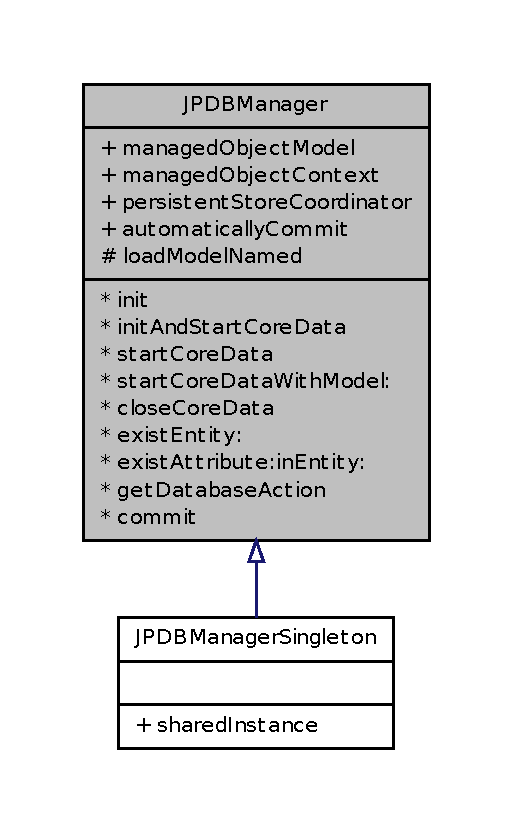
\includegraphics[width=246pt]{interface_j_p_d_b_manager__inherit__graph}
\end{center}
\end{figure}
\subsection*{Properties}
\begin{DoxyCompactItemize}
\item 
\hypertarget{interface_j_p_d_b_manager_a1325c5adbfd7d1952cdf0352fb064ba0}{
NSManagedObjectModel $\ast$ \hyperlink{interface_j_p_d_b_manager_a1325c5adbfd7d1952cdf0352fb064ba0}{managedObjectModel}}
\label{interface_j_p_d_b_manager_a1325c5adbfd7d1952cdf0352fb064ba0}

\begin{DoxyCompactList}\small\item\em Core Data Managed Object Model. \item\end{DoxyCompactList}\item 
\hypertarget{interface_j_p_d_b_manager_a29cf121d302956111efcc92ef6ebeb46}{
NSManagedObjectContext $\ast$ \hyperlink{interface_j_p_d_b_manager_a29cf121d302956111efcc92ef6ebeb46}{managedObjectContext}}
\label{interface_j_p_d_b_manager_a29cf121d302956111efcc92ef6ebeb46}

\begin{DoxyCompactList}\small\item\em Core Data Managed Object Context. \item\end{DoxyCompactList}\item 
\hypertarget{interface_j_p_d_b_manager_ac208712a609c528d79e7073211e4e658}{
NSPersistentStoreCoordinator $\ast$ \hyperlink{interface_j_p_d_b_manager_ac208712a609c528d79e7073211e4e658}{persistentStoreCoordinator}}
\label{interface_j_p_d_b_manager_ac208712a609c528d79e7073211e4e658}

\begin{DoxyCompactList}\small\item\em Core Data Persistent Store Coordinator. \item\end{DoxyCompactList}\item 
BOOL \hyperlink{interface_j_p_d_b_manager_a572163d38a033f106375cabe7b7748fa}{automaticallyCommit}
\begin{DoxyCompactList}\small\item\em Configure the manager to automatically commit every operation. \item\end{DoxyCompactList}\end{DoxyCompactItemize}
\subsection*{Init Methods}
\begin{DoxyCompactItemize}
\item 
(id) + \hyperlink{interface_j_p_d_b_manager_ad0fb072393aa238cb15f0fe71cae5034}{init}
\begin{DoxyCompactList}\small\item\em Init and Alloc the Database Manager Class. \item\end{DoxyCompactList}\item 
(id) + \hyperlink{interface_j_p_d_b_manager_add8b93f9565ad8b497a81d2cbdaa4301}{initAndStartCoreData}
\begin{DoxyCompactList}\small\item\em Init and Alloc the Database Manager Class. \item\end{DoxyCompactList}\end{DoxyCompactItemize}
\subsection*{Start and Stop Methods}
\begin{DoxyCompactItemize}
\item 
(id) -\/ \hyperlink{interface_j_p_d_b_manager_aef389466245327a533a7881fd2d54c52}{startCoreData}
\begin{DoxyCompactList}\small\item\em Start Core Data Databases. \item\end{DoxyCompactList}\item 
(id) -\/ \hyperlink{interface_j_p_d_b_manager_a3bf67f7522015669b34c6368bc836c55}{startCoreDataWithModel:}
\begin{DoxyCompactList}\small\item\em Start Core Data Databases. \item\end{DoxyCompactList}\item 
\hypertarget{interface_j_p_d_b_manager_ae3c82e3fa6e7da50efbd34357c5ddee4}{
(void) -\/ \hyperlink{interface_j_p_d_b_manager_ae3c82e3fa6e7da50efbd34357c5ddee4}{closeCoreData}}
\label{interface_j_p_d_b_manager_ae3c82e3fa6e7da50efbd34357c5ddee4}

\begin{DoxyCompactList}\small\item\em Close Core Data Databases, commit pendent updates and release resources. \item\end{DoxyCompactList}\end{DoxyCompactItemize}
\subsection*{Get Info Methods}
\begin{DoxyCompactItemize}
\item 
(BOOL) -\/ \hyperlink{interface_j_p_d_b_manager_a1d4236b0c842126f9ad6d30f53258a9f}{existEntity:}
\begin{DoxyCompactList}\small\item\em Test if specified Entity exist on the model. \item\end{DoxyCompactList}\item 
(BOOL) -\/ \hyperlink{interface_j_p_d_b_manager_a273547b21cbb031a49c35747e9240560}{existAttribute:inEntity:}
\begin{DoxyCompactList}\small\item\em Test if specified Attribute exist on specified Entity. \item\end{DoxyCompactList}\item 
(\hyperlink{interface_j_p_d_b_manager_action}{JPDBManagerAction} $\ast$) -\/ \hyperlink{interface_j_p_d_b_manager_a9eb7b1ed5ff3667b54a35a8d315cf689}{getDatabaseAction}
\begin{DoxyCompactList}\small\item\em Helper method to retrieve an \hyperlink{interface_j_p_d_b_manager_action}{Database Action} object. \item\end{DoxyCompactList}\end{DoxyCompactItemize}
\subsection*{Write Data Methods}
\begin{DoxyCompactItemize}
\item 
\hypertarget{interface_j_p_d_b_manager_ada5bce4a83f780c43da549468e1872dd}{
(void) -\/ \hyperlink{interface_j_p_d_b_manager_ada5bce4a83f780c43da549468e1872dd}{commit}}
\label{interface_j_p_d_b_manager_ada5bce4a83f780c43da549468e1872dd}

\begin{DoxyCompactList}\small\item\em Commit al pendent operations to the persistent store. \item\end{DoxyCompactList}\end{DoxyCompactItemize}


\subsection{Detailed Description}
Database Manager are one Facade around {\bfseries Core Data} classes that facilitate the main operations around the {\bfseries Core Data Framework{\bfseries . }}See the \hyperlink{basic_uses}{Basic Uses} to learn the basic concepts about this class. Also consult \hyperlink{errors}{Handling Errors} and \hyperlink{queries}{Performing Queries}. 

\subsection{Member Function Documentation}
\hypertarget{interface_j_p_d_b_manager_ad0fb072393aa238cb15f0fe71cae5034}{
\index{JPDBManager@{JPDBManager}!init@{init}}
\index{init@{init}!JPDBManager@{JPDBManager}}
\subsubsection[{init}]{\setlength{\rightskip}{0pt plus 5cm}+ (id) init 
\begin{DoxyParamCaption}
{}
\end{DoxyParamCaption}
}}
\label{interface_j_p_d_b_manager_ad0fb072393aa238cb15f0fe71cae5034}


Init and Alloc the Database Manager Class. 

\begin{DoxyReturn}{Returns}
One autoreleseable instance. 
\end{DoxyReturn}


Here is the caller graph for this function:
\nopagebreak
\begin{figure}[H]
\begin{center}
\leavevmode
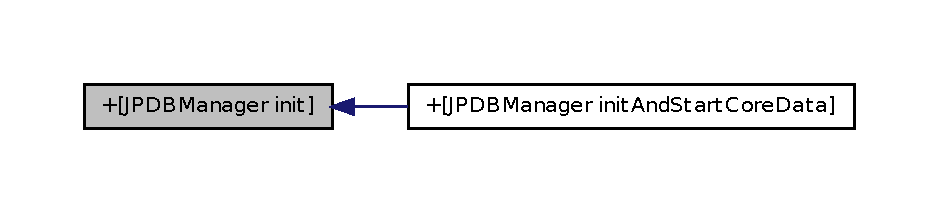
\includegraphics[width=400pt]{interface_j_p_d_b_manager_ad0fb072393aa238cb15f0fe71cae5034_icgraph}
\end{center}
\end{figure}


\hypertarget{interface_j_p_d_b_manager_add8b93f9565ad8b497a81d2cbdaa4301}{
\index{JPDBManager@{JPDBManager}!initAndStartCoreData@{initAndStartCoreData}}
\index{initAndStartCoreData@{initAndStartCoreData}!JPDBManager@{JPDBManager}}
\subsubsection[{initAndStartCoreData}]{\setlength{\rightskip}{0pt plus 5cm}+ (id) initAndStartCoreData 
\begin{DoxyParamCaption}
{}
\end{DoxyParamCaption}
}}
\label{interface_j_p_d_b_manager_add8b93f9565ad8b497a81d2cbdaa4301}


Init and Alloc the Database Manager Class. 

Automatically Start all Core Data Engine. \begin{DoxyReturn}{Returns}
One autoreleseable instance. 
\end{DoxyReturn}


Here is the call graph for this function:
\nopagebreak
\begin{figure}[H]
\begin{center}
\leavevmode
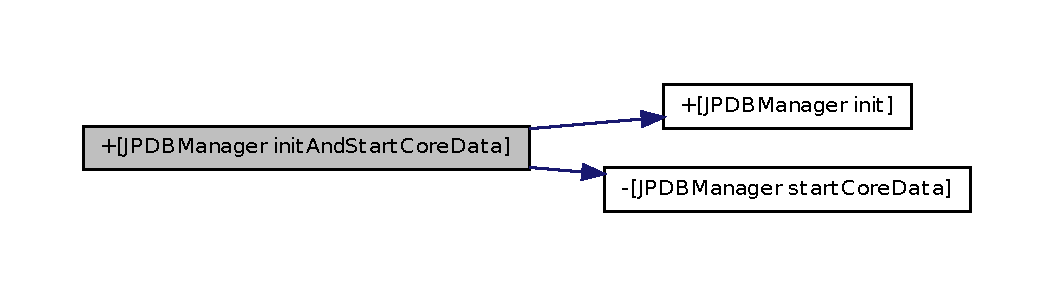
\includegraphics[width=400pt]{interface_j_p_d_b_manager_add8b93f9565ad8b497a81d2cbdaa4301_cgraph}
\end{center}
\end{figure}


\hypertarget{interface_j_p_d_b_manager_aef389466245327a533a7881fd2d54c52}{
\index{JPDBManager@{JPDBManager}!startCoreData@{startCoreData}}
\index{startCoreData@{startCoreData}!JPDBManager@{JPDBManager}}
\subsubsection[{startCoreData}]{\setlength{\rightskip}{0pt plus 5cm}-\/ (id) startCoreData 
\begin{DoxyParamCaption}
{}
\end{DoxyParamCaption}
}}
\label{interface_j_p_d_b_manager_aef389466245327a533a7881fd2d54c52}


Start Core Data Databases. 

Will merge ALL models in your bundle and try to recreate missed parameters. Use \hyperlink{interface_j_p_d_b_manager_a3bf67f7522015669b34c6368bc836c55}{startCoreDataWithModel:} if you need to use an specific model. 
\begin{DoxyExceptions}{Exceptions}
{\em An} & \hyperlink{errors_JPDBManagerStartException}{JPDBManagerStartException} exception is raised if some error ocurrs. See \hyperlink{errors}{Handling Errors} for more informations. \\
\hline
\end{DoxyExceptions}
\begin{DoxyReturn}{Returns}
Return itself. 
\end{DoxyReturn}


Here is the caller graph for this function:
\nopagebreak
\begin{figure}[H]
\begin{center}
\leavevmode
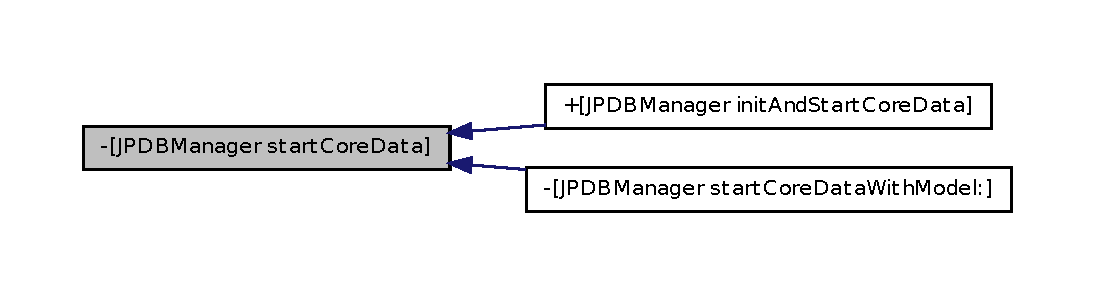
\includegraphics[width=400pt]{interface_j_p_d_b_manager_aef389466245327a533a7881fd2d54c52_icgraph}
\end{center}
\end{figure}


\hypertarget{interface_j_p_d_b_manager_a3bf67f7522015669b34c6368bc836c55}{
\index{JPDBManager@{JPDBManager}!startCoreDataWithModel:@{startCoreDataWithModel:}}
\index{startCoreDataWithModel:@{startCoreDataWithModel:}!JPDBManager@{JPDBManager}}
\subsubsection[{startCoreDataWithModel:}]{\setlength{\rightskip}{0pt plus 5cm}-\/ (id) startCoreDataWithModel: 
\begin{DoxyParamCaption}
\item[{dummy(NSString$\ast$)}]{modelName}
\end{DoxyParamCaption}
}}
\label{interface_j_p_d_b_manager_a3bf67f7522015669b34c6368bc836c55}


Start Core Data Databases. 


\begin{DoxyParams}{Parameters}
{\em modelName} & Specific Model Name. \\
\hline
\end{DoxyParams}

\begin{DoxyExceptions}{Exceptions}
{\em An} & \hyperlink{errors_JPDBManagerStartException}{JPDBManagerStartException} exception is raised if some error ocurrs. See \hyperlink{errors}{Handling Errors} for more informations. \\
\hline
\end{DoxyExceptions}
\begin{DoxyReturn}{Returns}
Return itself. 
\end{DoxyReturn}


Here is the call graph for this function:
\nopagebreak
\begin{figure}[H]
\begin{center}
\leavevmode
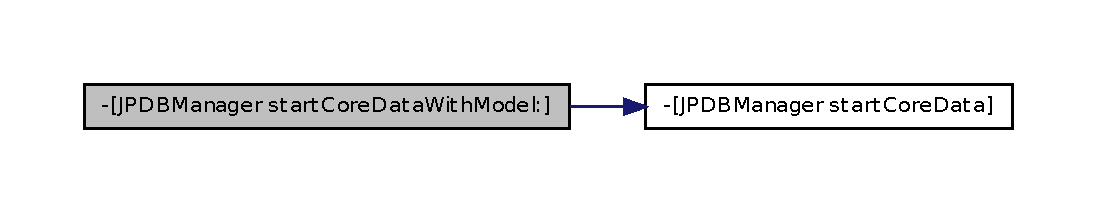
\includegraphics[width=400pt]{interface_j_p_d_b_manager_a3bf67f7522015669b34c6368bc836c55_cgraph}
\end{center}
\end{figure}


\hypertarget{interface_j_p_d_b_manager_a1d4236b0c842126f9ad6d30f53258a9f}{
\index{JPDBManager@{JPDBManager}!existEntity:@{existEntity:}}
\index{existEntity:@{existEntity:}!JPDBManager@{JPDBManager}}
\subsubsection[{existEntity:}]{\setlength{\rightskip}{0pt plus 5cm}-\/ (BOOL) existEntity: 
\begin{DoxyParamCaption}
\item[{dummy(NSString$\ast$)}]{anEntityName}
\end{DoxyParamCaption}
}}
\label{interface_j_p_d_b_manager_a1d4236b0c842126f9ad6d30f53258a9f}


Test if specified Entity exist on the model. 


\begin{DoxyParams}{Parameters}
{\em anEntityName} & The Entity Name. \\
\hline
\end{DoxyParams}
\begin{DoxyReturn}{Returns}
YES if specified Entity exist on the model. 
\end{DoxyReturn}
\hypertarget{interface_j_p_d_b_manager_a273547b21cbb031a49c35747e9240560}{
\index{JPDBManager@{JPDBManager}!existAttribute:inEntity:@{existAttribute:inEntity:}}
\index{existAttribute:inEntity:@{existAttribute:inEntity:}!JPDBManager@{JPDBManager}}
\subsubsection[{existAttribute:inEntity:}]{\setlength{\rightskip}{0pt plus 5cm}-\/ (BOOL) existAttribute: 
\begin{DoxyParamCaption}
\item[{dummy(NSString$\ast$)}]{anAttributeName}
\item[{inEntity:(NSString$\ast$)}]{anEntityName}
\end{DoxyParamCaption}
}}
\label{interface_j_p_d_b_manager_a273547b21cbb031a49c35747e9240560}


Test if specified Attribute exist on specified Entity. 


\begin{DoxyParams}{Parameters}
{\em anAttributeName} & The Attribute name. \\
\hline
{\em anEntityName} & The Entity name. \\
\hline
\end{DoxyParams}
\begin{DoxyReturn}{Returns}
{\bfseries YES} if specified Attribute exist on specified Entity. 
\end{DoxyReturn}
\hypertarget{interface_j_p_d_b_manager_a9eb7b1ed5ff3667b54a35a8d315cf689}{
\index{JPDBManager@{JPDBManager}!getDatabaseAction@{getDatabaseAction}}
\index{getDatabaseAction@{getDatabaseAction}!JPDBManager@{JPDBManager}}
\subsubsection[{getDatabaseAction}]{\setlength{\rightskip}{0pt plus 5cm}-\/ ({\bf JPDBManagerAction} $\ast$) getDatabaseAction 
\begin{DoxyParamCaption}
{}
\end{DoxyParamCaption}
}}
\label{interface_j_p_d_b_manager_a9eb7b1ed5ff3667b54a35a8d315cf689}


Helper method to retrieve an \hyperlink{interface_j_p_d_b_manager_action}{Database Action} object. 

The manager is automatically associcated to this object. 

Here is the call graph for this function:
\nopagebreak
\begin{figure}[H]
\begin{center}
\leavevmode
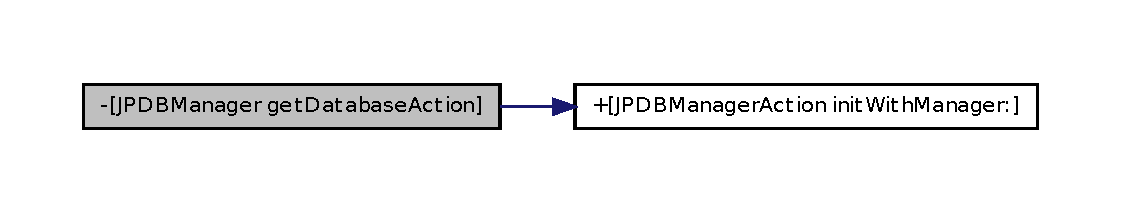
\includegraphics[width=400pt]{interface_j_p_d_b_manager_a9eb7b1ed5ff3667b54a35a8d315cf689_cgraph}
\end{center}
\end{figure}




\subsection{Property Documentation}
\hypertarget{interface_j_p_d_b_manager_a572163d38a033f106375cabe7b7748fa}{
\index{JPDBManager@{JPDBManager}!automaticallyCommit@{automaticallyCommit}}
\index{automaticallyCommit@{automaticallyCommit}!JPDBManager@{JPDBManager}}
\subsubsection[{automaticallyCommit}]{\setlength{\rightskip}{0pt plus 5cm}-\/ (BOOL) automaticallyCommit\hspace{0.3cm}{\ttfamily  \mbox{[}read, write, assign\mbox{]}}}}
\label{interface_j_p_d_b_manager_a572163d38a033f106375cabe7b7748fa}


Configure the manager to automatically commit every operation. 

Default value is {\bfseries NO}. See \hyperlink{basic_uses}{Basic Uses} for more information. 

The documentation for this class was generated from the following files:\begin{DoxyCompactItemize}
\item 
/Users/Paulo/Projects/JUMP/JUMPDatabase/Headers/JPDBManager.h\item 
/Users/Paulo/Projects/JUMP/JUMPDatabase/Sources/JPDBManager.m\end{DoxyCompactItemize}

\hypertarget{interface_j_p_d_b_manager_action}{
\section{JPDBManagerAction Class Reference}
\label{interface_j_p_d_b_manager_action}\index{JPDBManagerAction@{JPDBManagerAction}}
}


{\bfseries Database Manager Action} pack all data and settings to perform some database operation.  




{\ttfamily \#import $<$JPDBManagerAction.h$>$}

\subsection*{Properties}
\begin{DoxyCompactItemize}
\item 
\hypertarget{interface_j_p_d_b_manager_action_a705cfdcdfd4ff48deff4ba42928412b9}{
NSString $\ast$ \hyperlink{interface_j_p_d_b_manager_action_a705cfdcdfd4ff48deff4ba42928412b9}{entity}}
\label{interface_j_p_d_b_manager_action_a705cfdcdfd4ff48deff4ba42928412b9}

\begin{DoxyCompactList}\small\item\em The entity to perform this action. \item\end{DoxyCompactList}\item 
\hypertarget{interface_j_p_d_b_manager_action_af2476369c483c826653f8b7d1721c452}{
NSString $\ast$ \hyperlink{interface_j_p_d_b_manager_action_af2476369c483c826653f8b7d1721c452}{fetchTemplate}}
\label{interface_j_p_d_b_manager_action_af2476369c483c826653f8b7d1721c452}

\begin{DoxyCompactList}\small\item\em The Fetch Template to perform this action. \item\end{DoxyCompactList}\item 
\hypertarget{interface_j_p_d_b_manager_action_a8832555fcf8837ece9ded4a9ba408fd4}{
NSMutableDictionary $\ast$ \hyperlink{interface_j_p_d_b_manager_action_a8832555fcf8837ece9ded4a9ba408fd4}{variablesListAndValues}}
\label{interface_j_p_d_b_manager_action_a8832555fcf8837ece9ded4a9ba408fd4}

\begin{DoxyCompactList}\small\item\em Values to replace on the pre formatted Fetch Template. \item\end{DoxyCompactList}\item 
\hypertarget{interface_j_p_d_b_manager_action_a354db0f8d4e9039eb7e4095526786ade}{
NSMutableArray $\ast$ \hyperlink{interface_j_p_d_b_manager_action_a354db0f8d4e9039eb7e4095526786ade}{sortDescriptors}}
\label{interface_j_p_d_b_manager_action_a354db0f8d4e9039eb7e4095526786ade}

\begin{DoxyCompactList}\small\item\em Array of Sort Descriptors ({\bfseries NSSortDescriptor}) to sort the result of this acion. \item\end{DoxyCompactList}\item 
\hypertarget{interface_j_p_d_b_manager_action_a675723939f92d5da2a8280e83bd0e1f0}{
\hyperlink{interface_j_p_d_b_manager}{JPDBManager} $\ast$ \hyperlink{interface_j_p_d_b_manager_action_a675723939f92d5da2a8280e83bd0e1f0}{manager}}
\label{interface_j_p_d_b_manager_action_a675723939f92d5da2a8280e83bd0e1f0}

\begin{DoxyCompactList}\small\item\em Instance of the Manager to perform this Database Action. \item\end{DoxyCompactList}\item 
BOOL \hyperlink{interface_j_p_d_b_manager_action_ad0060c13ad4e89eb23c60ad123250505}{commitTransaction}
\begin{DoxyCompactList}\small\item\em Set if the Manager should commit this transaction immediatelly or not. \item\end{DoxyCompactList}\item 
BOOL \hyperlink{interface_j_p_d_b_manager_action_ae603fd48edaea29a115b90a19f440ab8}{returnObjectsAsFault}
\begin{DoxyCompactList}\small\item\em Define if the Result objects of some query should be as Core Data Fault. \item\end{DoxyCompactList}\item 
BOOL \hyperlink{interface_j_p_d_b_manager_action_a0e153817018f1c41c7fa6bd5780ef09a}{ascendingOrder}
\begin{DoxyCompactList}\small\item\em Define if the order of the results of some query should be Ascending or Descending. \item\end{DoxyCompactList}\item 
BOOL \hyperlink{interface_j_p_d_b_manager_action_aecdffb5193789cbd3e4704e71c90972c}{returnActionAsArray}
\begin{DoxyCompactList}\small\item\em Set if the Result of this action should be an {\bfseries NSArray} or an {\bfseries NSFetchedResultsController} object. \item\end{DoxyCompactList}\end{DoxyCompactItemize}
\subsection*{Init Methods}
\begin{DoxyCompactItemize}
\item 
(id) + \hyperlink{interface_j_p_d_b_manager_action_a95c4b89cda57087f508cee1b3aacac59}{initWithManager:}
\begin{DoxyCompactList}\small\item\em Init with an \hyperlink{interface_j_p_d_b_manager}{Database Manager} to process this Database Action. \item\end{DoxyCompactList}\item 
(id) -\/ \hyperlink{interface_j_p_d_b_manager_action_a95c4b89cda57087f508cee1b3aacac59}{initWithManager:}
\begin{DoxyCompactList}\small\item\em Init with an \hyperlink{interface_j_p_d_b_manager}{Database Manager} to process this Database Action. \item\end{DoxyCompactList}\end{DoxyCompactItemize}
\subsection*{Set Query Limits}
\begin{DoxyCompactItemize}
\item 
int \hyperlink{interface_j_p_d_b_manager_action_ad679e0229dbddd7d5c87a6348d33fc9e}{startFetchInLine}
\begin{DoxyCompactList}\small\item\em Set the initial row result to return from Query Methods results. \item\end{DoxyCompactList}\item 
int \hyperlink{interface_j_p_d_b_manager_action_a768d19efb483654b753bdc3a8bf1a197}{limitFetchResults}
\begin{DoxyCompactList}\small\item\em Set the maximum rows to return from Query Methods results. \item\end{DoxyCompactList}\item 
\hypertarget{interface_j_p_d_b_manager_action_aed8e76eb4ccf0c1794a3f0d4468d6c16}{
(void) -\/ \hyperlink{interface_j_p_d_b_manager_action_aed8e76eb4ccf0c1794a3f0d4468d6c16}{setStartFetchInLine:setLimitFetchResults:}}
\label{interface_j_p_d_b_manager_action_aed8e76eb4ccf0c1794a3f0d4468d6c16}

\begin{DoxyCompactList}\small\item\em Convenient method to set the \hyperlink{interface_j_p_d_b_manager_action_ad679e0229dbddd7d5c87a6348d33fc9e}{startFetchInLine} and \hyperlink{interface_j_p_d_b_manager_action_a768d19efb483654b753bdc3a8bf1a197}{limitFetchResults} properties at the same time. \item\end{DoxyCompactList}\item 
\hypertarget{interface_j_p_d_b_manager_action_aac879451f1f7769f2c22061f0b3d9479}{
(void) -\/ \hyperlink{interface_j_p_d_b_manager_action_aac879451f1f7769f2c22061f0b3d9479}{resetFetchLimits}}
\label{interface_j_p_d_b_manager_action_aac879451f1f7769f2c22061f0b3d9479}

\begin{DoxyCompactList}\small\item\em Reset the default Fetch Limits values. \item\end{DoxyCompactList}\item 
\hypertarget{interface_j_p_d_b_manager_action_a2217de1fa0fd2e0302200fa745e2fdf0}{
(void) -\/ \hyperlink{interface_j_p_d_b_manager_action_a2217de1fa0fd2e0302200fa745e2fdf0}{resetDefaultValues}}
\label{interface_j_p_d_b_manager_action_a2217de1fa0fd2e0302200fa745e2fdf0}

\begin{DoxyCompactList}\small\item\em Reset this Action Settings to default values. \item\end{DoxyCompactList}\end{DoxyCompactItemize}
\subsection*{Action Data Methods}
\begin{DoxyCompactItemize}
\item 
(id) -\/ \hyperlink{interface_j_p_d_b_manager_action_aefef71fec8be541c06102b052e0b3c04}{applyEntity:}
\begin{DoxyCompactList}\small\item\em Set an Entity to perform this action. \item\end{DoxyCompactList}\item 
(id) -\/ \hyperlink{interface_j_p_d_b_manager_action_ac21e1e26b08f892d10e6a434f03958e6}{applyFetchTemplate:}
\begin{DoxyCompactList}\small\item\em Set an Fetch Template name to perform this action. \item\end{DoxyCompactList}\item 
(id) -\/ \hyperlink{interface_j_p_d_b_manager_action_a1f0599e3441beb8b911b9d0f73c89329}{applyFetchReplaceWithDictionary:}
\begin{DoxyCompactList}\small\item\em Set the Values to replace on the pre formatted Fetch Template. \item\end{DoxyCompactList}\item 
(id) -\/ \hyperlink{interface_j_p_d_b_manager_action_a326f7abe356e685297cfa32460dd7101}{applyFetchReplaceWithVariables:}
\begin{DoxyCompactList}\small\item\em Set the Values to replace on the pre formatted Fetch Template. \item\end{DoxyCompactList}\item 
\hypertarget{interface_j_p_d_b_manager_action_a11e31543021bbf876a3d83b16dce0d75}{
(id) -\/ {\bfseries applyPredicate:}}
\label{interface_j_p_d_b_manager_action_a11e31543021bbf876a3d83b16dce0d75}

\item 
\hypertarget{interface_j_p_d_b_manager_action_a949b92949f557892131e135a5cbbffde}{
(id) -\/ \hyperlink{interface_j_p_d_b_manager_action_a949b92949f557892131e135a5cbbffde}{runAction}}
\label{interface_j_p_d_b_manager_action_a949b92949f557892131e135a5cbbffde}

\begin{DoxyCompactList}\small\item\em Run this action on the associated \hyperlink{interface_j_p_d_b_manager}{JPDBManager} Database Manager. \item\end{DoxyCompactList}\end{DoxyCompactItemize}
\subsection*{Order Keys Methods}
\begin{DoxyCompactItemize}
\item 
(id) -\/ \hyperlink{interface_j_p_d_b_manager_action_ac7b38fbbab436a50344de7e5c61238b8}{applyArrayOfSortDescriptors:}
\begin{DoxyCompactList}\small\item\em Set the Key attributes to sort the result of this acion. \item\end{DoxyCompactList}\item 
(id) -\/ \hyperlink{interface_j_p_d_b_manager_action_aab038bf441025fe2d6615a49d67d6477}{applyOrderKeys:}
\begin{DoxyCompactList}\small\item\em Set the Key attributes to sort the result of this acion. \item\end{DoxyCompactList}\item 
(id) -\/ \hyperlink{interface_j_p_d_b_manager_action_a432c1012382e6baa4c76c051a524881e}{applyOrderKey:}
\begin{DoxyCompactList}\small\item\em Set the Key attribute to sort the result of this acion. \item\end{DoxyCompactList}\item 
(id) -\/ \hyperlink{interface_j_p_d_b_manager_action_a2ed39b1660529638ea1596cfea71580d}{addOrderKey:}
\begin{DoxyCompactList}\small\item\em Add a new Key attribute to sort the result of this action. \item\end{DoxyCompactList}\item 
(void) -\/ \hyperlink{interface_j_p_d_b_manager_action_a5ca5bdf039427760eb017fd51575d0e2}{removeOrderKey:}
\begin{DoxyCompactList}\small\item\em Remove an Key attribute from the sorter list. \item\end{DoxyCompactList}\end{DoxyCompactItemize}
\subsection*{Query All Data Methods}
\begin{DoxyCompactItemize}
\item 
(id) -\/ \hyperlink{interface_j_p_d_b_manager_action_a367267b639633531a6e44c6b7857cfd0}{queryAllDataFromEntity:}
\begin{DoxyCompactList}\small\item\em Query all data of the specified Entity. \item\end{DoxyCompactList}\item 
(id) -\/ \hyperlink{interface_j_p_d_b_manager_action_a41146d672b6282be3eb7ef37dffe17d0}{queryAllDataFromEntity:orderWithKey:}
\begin{DoxyCompactList}\small\item\em Query all data of the specified Entity. \item\end{DoxyCompactList}\item 
(id) -\/ \hyperlink{interface_j_p_d_b_manager_action_ad26a0af6246a53d8497178371308e28d}{queryAllDataFromEntity:orderWithKeys:}
\begin{DoxyCompactList}\small\item\em Query all data of the specified Entity. \item\end{DoxyCompactList}\end{DoxyCompactItemize}
\subsection*{Query Data With Fetch Templates Methods}
\begin{DoxyCompactItemize}
\item 
(id) -\/ \hyperlink{interface_j_p_d_b_manager_action_a37853bbac86c15f62981187bd9d7bcfc}{queryEntity:withFetchTemplate:}
\begin{DoxyCompactList}\small\item\em Query specified Entity using one specified Fetch Template name. \item\end{DoxyCompactList}\item 
(id) -\/ \hyperlink{interface_j_p_d_b_manager_action_aa857b7593c614e34728ba1c346774e47}{queryEntity:withFetchTemplate:orderWithKey:}
\begin{DoxyCompactList}\small\item\em Query specified Entity using one specified Fetch Template name. \item\end{DoxyCompactList}\item 
(id) -\/ \hyperlink{interface_j_p_d_b_manager_action_ac9cc8404e73e1cb38ce0cc50cbac3ecd}{queryEntity:withFetchTemplate:orderWithKeys:}
\begin{DoxyCompactList}\small\item\em Query specified Entity using one specified Fetch Template name. \item\end{DoxyCompactList}\end{DoxyCompactItemize}
\subsection*{Query Data With Fetch Templates and Fetch Parameters Methods}
\begin{DoxyCompactItemize}
\item 
(id) -\/ \hyperlink{interface_j_p_d_b_manager_action_aac56b1fa8bf99688b4ea5f117036eff0}{queryEntity:withFetchTemplate:withVariables:}
\begin{DoxyCompactList}\small\item\em Query specified Entity using one specified Fetch Template name. \item\end{DoxyCompactList}\item 
(id) -\/ \hyperlink{interface_j_p_d_b_manager_action_a3044583007eb7aa00185a5da222acc40}{queryEntity:withFetchTemplate:orderWithKey:withVariables:}
\begin{DoxyCompactList}\small\item\em Query specified Entity using one specified Fetch Template name. \item\end{DoxyCompactList}\item 
(id) -\/ \hyperlink{interface_j_p_d_b_manager_action_ae32ca03d7ce37116f5c9e292e368bf8f}{queryEntity:withFetchTemplate:replaceFetchWithDictionary:}
\begin{DoxyCompactList}\small\item\em Query specified Entity using one specified Fetch Template name. \item\end{DoxyCompactList}\item 
(id) -\/ \hyperlink{interface_j_p_d_b_manager_action_aef6b587a0260a962b3ba9946d5590997}{queryEntity:withFetchTemplate:replaceFetchWithDictionary:orderWithKey:}
\begin{DoxyCompactList}\small\item\em Query specified Entity using one specified Fetch Template name. \item\end{DoxyCompactList}\item 
(id) -\/ \hyperlink{interface_j_p_d_b_manager_action_ac04b76b32d39ae9b412f99b3ac620a86}{queryEntity:withFetchTemplate:replaceFetchWithDictionary:orderWithKeys:}
\begin{DoxyCompactList}\small\item\em Query specified Entity using one specified Fetch Template name. \item\end{DoxyCompactList}\item 
(id) -\/ \hyperlink{interface_j_p_d_b_manager_action_ad9f87e94c40f183732a44fd181ec96f6}{queryEntity:withFetchTemplate:replaceFetchWithDictionary:arrayOfSortDescriptors:}
\begin{DoxyCompactList}\small\item\em Query specified Entity using one specified Fetch Template name. \item\end{DoxyCompactList}\item 
\hypertarget{interface_j_p_d_b_manager_action_a22a107d745d907acf845ab0e2528f18e}{
(id) -\/ {\bfseries queryEntity:withFetchTemplate:replaceFetchWithDictionary:arrayOfSortDescriptors:customPredicate:}}
\label{interface_j_p_d_b_manager_action_a22a107d745d907acf845ab0e2528f18e}

\end{DoxyCompactItemize}
\subsection*{Query Data Methods With Custom Predicates}
\begin{DoxyCompactItemize}
\item 
(id) -\/ \hyperlink{interface_j_p_d_b_manager_action_a0b4bbc0a957856f7e0166d58f987e8dc}{queryEntity:withPredicate:}
\begin{DoxyCompactList}\small\item\em Query specified Entity using one custom NSPredicate Object. \item\end{DoxyCompactList}\item 
(id) -\/ \hyperlink{interface_j_p_d_b_manager_action_a59b25a33e515e04dbf7e7d83855e86d1}{queryEntity:withPredicate:orderWithKey:}
\begin{DoxyCompactList}\small\item\em Query specified Entity using one custom NSPredicate Object. \item\end{DoxyCompactList}\item 
(id) -\/ \hyperlink{interface_j_p_d_b_manager_action_a8b9de476586b7352658c07c6f9b92bd9}{queryEntity:withPredicate:orderWithKeys:}
\begin{DoxyCompactList}\small\item\em Query specified Entity using one custom NSPredicate Object. \item\end{DoxyCompactList}\item 
(id) -\/ \hyperlink{interface_j_p_d_b_manager_action_aa7020d4c7938f259bab678b4c9b0a056}{queryEntity:withPredicate:arrayOfSortDescriptors:}
\begin{DoxyCompactList}\small\item\em Query specified Entity using one custom NSPredicate Object. \item\end{DoxyCompactList}\end{DoxyCompactItemize}
\subsection*{Remove Data Methods}
\begin{DoxyCompactItemize}
\item 
(void) -\/ \hyperlink{interface_j_p_d_b_manager_action_ac566a65fcbfa1026f42954648d60e6b8}{deleteRecord:}
\begin{DoxyCompactList}\small\item\em Delete specified Record from his Entity on the Database. \item\end{DoxyCompactList}\item 
(void) -\/ \hyperlink{interface_j_p_d_b_manager_action_a7a8d41ed1791761c1996af5d031e41a7}{deleteRecord:andCommit:}
\begin{DoxyCompactList}\small\item\em Delete specified Record from his Entity on the Database. \item\end{DoxyCompactList}\item 
(void) -\/ \hyperlink{interface_j_p_d_b_manager_action_af85b28a738631615ad0e4030500ce71a}{deleteRecordsFromEntity:withFetchTemplate:}
\begin{DoxyCompactList}\small\item\em Delete all records queried by the specified Fetch Template. \item\end{DoxyCompactList}\item 
(void) -\/ \hyperlink{interface_j_p_d_b_manager_action_a1a7a137d9a6617366523dca5a59174a0}{deleteAllRecordsFromEntity:}
\begin{DoxyCompactList}\small\item\em Delete all Records from specified Entity. \item\end{DoxyCompactList}\end{DoxyCompactItemize}
\subsection*{Write Data Methods}
\begin{DoxyCompactItemize}
\item 
(id) -\/ \hyperlink{interface_j_p_d_b_manager_action_a64efbdc0e61408df85b45629141871e6}{createNewRecordForEntity:}
\begin{DoxyCompactList}\small\item\em Create and return a new record for specified Entity. \item\end{DoxyCompactList}\end{DoxyCompactItemize}


\subsection{Detailed Description}
{\bfseries Database Manager Action} pack all data and settings to perform some database operation. Database operations isn't called directy to the manager. Instead we create one instance of the \hyperlink{interface_j_p_d_b_manager_action}{JPDBManagerAction} class, configure the data and settings to perform some \href{http://en.wikipedia.org/wiki/Create,_read,_update_and_delete}{\tt CRUD} operation and finally run this action. Yes, looks like a lot of work, but actually is not. Let's see some examples: 
\begin{DoxyCode}
 id newRecord = [JPDatabaseManager createNewRecordForEntity:@"MyEntity"];
\end{DoxyCode}
 This is was really simple, isn't? Let's see this same operation on a more custom fashion: 
\begin{DoxyCode}
 JPDBManagerAction *anAction = [[JPDBManagerSingleton sharedInstance] 
      getDatabaseAction];
 [anAction setCommitTransaction:YES];
 id newRecord = [anAction createNewRecordForEntity:@"MyEntity"];
\end{DoxyCode}
 Well this looks a litle bit more complicated. Let's understand this two processes: The first one uses the {\bfseries JPDatabaseManager} convenient macro shortcut that returns an \hyperlink{interface_j_p_d_b_manager_action}{JPDBManagerAction} instance and perform this method in only one pass, is pure convenience. This macro is declared in the \hyperlink{_j_p_d_b_manager_definitions_8h_source}{JPDBManagerDefinitions.h} file. \par
 \par
 The second way needs more steps, but you should use that way when you need more control of the all process, for example, you can configure if you want to automatically commit the operation or create some more dinamically code on your database operations. \par
 

\subsection{Member Function Documentation}
\hypertarget{interface_j_p_d_b_manager_action_a95c4b89cda57087f508cee1b3aacac59}{
\index{JPDBManagerAction@{JPDBManagerAction}!initWithManager:@{initWithManager:}}
\index{initWithManager:@{initWithManager:}!JPDBManagerAction@{JPDBManagerAction}}
\subsubsection[{initWithManager:}]{\setlength{\rightskip}{0pt plus 5cm}+ (id) initWithManager: 
\begin{DoxyParamCaption}
\item[{dummy({\bf JPDBManager}$\ast$)}]{anManager}
\end{DoxyParamCaption}
}}
\label{interface_j_p_d_b_manager_action_a95c4b89cda57087f508cee1b3aacac59}


Init with an \hyperlink{interface_j_p_d_b_manager}{Database Manager} to process this Database Action. 


\begin{DoxyParams}{Parameters}
{\em anManager} & An \hyperlink{interface_j_p_d_b_manager}{Database Manager  An autoreleseable instance. }\\
\hline
\end{DoxyParams}


Here is the caller graph for this function:
\nopagebreak
\begin{figure}[H]
\begin{center}
\leavevmode
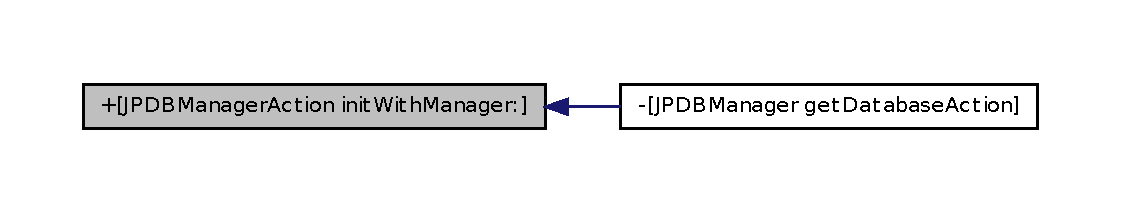
\includegraphics[width=400pt]{interface_j_p_d_b_manager_action_a95c4b89cda57087f508cee1b3aacac59_icgraph}
\end{center}
\end{figure}


\hypertarget{interface_j_p_d_b_manager_action_a95c4b89cda57087f508cee1b3aacac59}{
\index{JPDBManagerAction@{JPDBManagerAction}!initWithManager:@{initWithManager:}}
\index{initWithManager:@{initWithManager:}!JPDBManagerAction@{JPDBManagerAction}}
\subsubsection[{initWithManager:}]{\setlength{\rightskip}{0pt plus 5cm}-\/ (id) initWithManager: 
\begin{DoxyParamCaption}
\item[{dummy({\bf JPDBManager} $\ast$)}]{anManager}
\end{DoxyParamCaption}
}}
\label{interface_j_p_d_b_manager_action_a95c4b89cda57087f508cee1b3aacac59}


Init with an \hyperlink{interface_j_p_d_b_manager}{Database Manager} to process this Database Action. 


\begin{DoxyParams}{Parameters}
{\em anManager} & An \hyperlink{interface_j_p_d_b_manager}{Database Manager  An retained instance. }\\
\hline
\end{DoxyParams}
\hypertarget{interface_j_p_d_b_manager_action_aefef71fec8be541c06102b052e0b3c04}{
\index{JPDBManagerAction@{JPDBManagerAction}!applyEntity:@{applyEntity:}}
\index{applyEntity:@{applyEntity:}!JPDBManagerAction@{JPDBManagerAction}}
\subsubsection[{applyEntity:}]{\setlength{\rightskip}{0pt plus 5cm}-\/ (id) applyEntity: 
\begin{DoxyParamCaption}
\item[{dummy(NSString$\ast$)}]{anEntity}
\end{DoxyParamCaption}
}}
\label{interface_j_p_d_b_manager_action_aefef71fec8be541c06102b052e0b3c04}


Set an Entity to perform this action. 


\begin{DoxyParams}{Parameters}
{\em anEntityName} & The Entity Name. \\
\hline
\end{DoxyParams}
\begin{DoxyReturn}{Returns}
Return itself. 
\end{DoxyReturn}


Here is the caller graph for this function:
\nopagebreak
\begin{figure}[H]
\begin{center}
\leavevmode
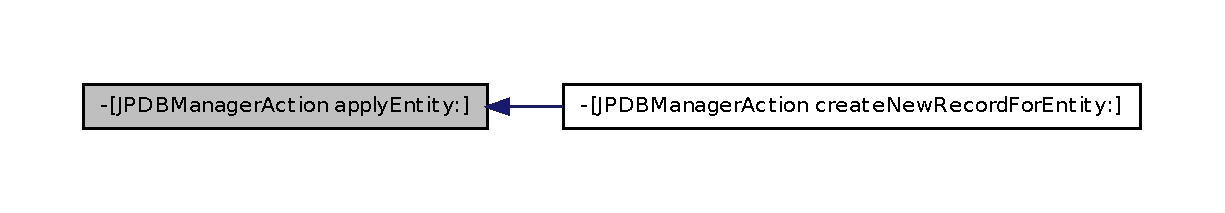
\includegraphics[width=400pt]{interface_j_p_d_b_manager_action_aefef71fec8be541c06102b052e0b3c04_icgraph}
\end{center}
\end{figure}


\hypertarget{interface_j_p_d_b_manager_action_ac21e1e26b08f892d10e6a434f03958e6}{
\index{JPDBManagerAction@{JPDBManagerAction}!applyFetchTemplate:@{applyFetchTemplate:}}
\index{applyFetchTemplate:@{applyFetchTemplate:}!JPDBManagerAction@{JPDBManagerAction}}
\subsubsection[{applyFetchTemplate:}]{\setlength{\rightskip}{0pt plus 5cm}-\/ (id) applyFetchTemplate: 
\begin{DoxyParamCaption}
\item[{dummy(NSString$\ast$)}]{anFetchTemplate}
\end{DoxyParamCaption}
}}
\label{interface_j_p_d_b_manager_action_ac21e1e26b08f892d10e6a434f03958e6}


Set an Fetch Template name to perform this action. 


\begin{DoxyParams}{Parameters}
{\em anFetchRequest} & An Fetch Template to perform the query. \\
\hline
\end{DoxyParams}
\begin{DoxyReturn}{Returns}
Return itself. 
\end{DoxyReturn}
\hypertarget{interface_j_p_d_b_manager_action_a1f0599e3441beb8b911b9d0f73c89329}{
\index{JPDBManagerAction@{JPDBManagerAction}!applyFetchReplaceWithDictionary:@{applyFetchReplaceWithDictionary:}}
\index{applyFetchReplaceWithDictionary:@{applyFetchReplaceWithDictionary:}!JPDBManagerAction@{JPDBManagerAction}}
\subsubsection[{applyFetchReplaceWithDictionary:}]{\setlength{\rightskip}{0pt plus 5cm}-\/ (id) applyFetchReplaceWithDictionary: 
\begin{DoxyParamCaption}
\item[{dummy(NSDictionary$\ast$)}]{anDictionary}
\end{DoxyParamCaption}
}}
\label{interface_j_p_d_b_manager_action_a1f0599e3441beb8b911b9d0f73c89329}


Set the Values to replace on the pre formatted Fetch Template. 


\begin{DoxyParams}{Parameters}
{\em anDictionary} & An Dictionary with Keys and Values to replace on the pre formatted Fetch Template \\
\hline
\end{DoxyParams}
\begin{DoxyReturn}{Returns}
Return itself. 
\end{DoxyReturn}


Here is the caller graph for this function:
\nopagebreak
\begin{figure}[H]
\begin{center}
\leavevmode
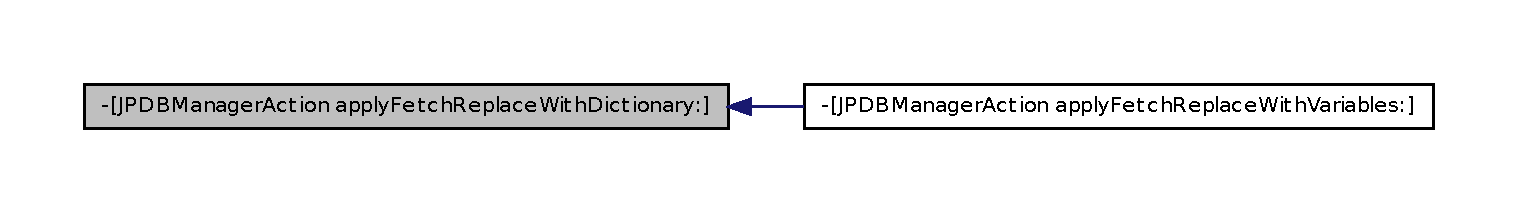
\includegraphics[width=400pt]{interface_j_p_d_b_manager_action_a1f0599e3441beb8b911b9d0f73c89329_icgraph}
\end{center}
\end{figure}


\hypertarget{interface_j_p_d_b_manager_action_a326f7abe356e685297cfa32460dd7101}{
\index{JPDBManagerAction@{JPDBManagerAction}!applyFetchReplaceWithVariables:@{applyFetchReplaceWithVariables:}}
\index{applyFetchReplaceWithVariables:@{applyFetchReplaceWithVariables:}!JPDBManagerAction@{JPDBManagerAction}}
\subsubsection[{applyFetchReplaceWithVariables:}]{\setlength{\rightskip}{0pt plus 5cm}-\/ (id) applyFetchReplaceWithVariables: 
\begin{DoxyParamCaption}
\item[{dummy(id)}]{variableList}
\item[{,}]{NS\_\-REQUIRES\_\-NIL\_\-TERMINATION}
\end{DoxyParamCaption}
}}
\label{interface_j_p_d_b_manager_action_a326f7abe356e685297cfa32460dd7101}


Set the Values to replace on the pre formatted Fetch Template. 


\begin{DoxyParams}{Parameters}
{\em variableList} & Keys and Values to replace on the pre formatted Fetch Template.\par
 {\bfseries Example:}\par
 
\begin{DoxyCode}
 [anAction applyFetchReplaceWithVariables:@"value1", @"key1", @"value2", @"key2",
       nil];
\end{DoxyCode}
 \\
\hline
\end{DoxyParams}
\begin{DoxyReturn}{Returns}
Return itself. 
\end{DoxyReturn}


Here is the call graph for this function:
\nopagebreak
\begin{figure}[H]
\begin{center}
\leavevmode
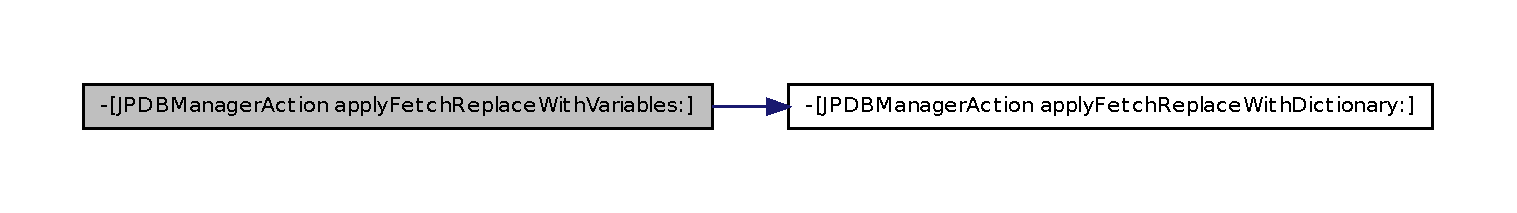
\includegraphics[width=400pt]{interface_j_p_d_b_manager_action_a326f7abe356e685297cfa32460dd7101_cgraph}
\end{center}
\end{figure}


\hypertarget{interface_j_p_d_b_manager_action_ac7b38fbbab436a50344de7e5c61238b8}{
\index{JPDBManagerAction@{JPDBManagerAction}!applyArrayOfSortDescriptors:@{applyArrayOfSortDescriptors:}}
\index{applyArrayOfSortDescriptors:@{applyArrayOfSortDescriptors:}!JPDBManagerAction@{JPDBManagerAction}}
\subsubsection[{applyArrayOfSortDescriptors:}]{\setlength{\rightskip}{0pt plus 5cm}-\/ (id) applyArrayOfSortDescriptors: 
\begin{DoxyParamCaption}
\item[{dummy(NSArray$\ast$)}]{anArray}
\end{DoxyParamCaption}
}}
\label{interface_j_p_d_b_manager_action_ac7b38fbbab436a50344de7e5c61238b8}


Set the Key attributes to sort the result of this acion. 


\begin{DoxyParams}{Parameters}
{\em anArrayOfSortDescriptors} & An Array with defined {\bfseries NSSortDescriptors} to sort the result. \\
\hline
\end{DoxyParams}

\begin{DoxyExceptions}{Exceptions}
{\em An} & \hyperlink{errors_JPDBManagerActionException}{JPDBManagerActionException} exception if the array contains an objects that doesn't is an {\bfseries NSSortDescriptors}. See \hyperlink{errors}{Handling Errors} for more informations. \\
\hline
\end{DoxyExceptions}
\begin{DoxyReturn}{Returns}
Return itself. 
\end{DoxyReturn}


Here is the caller graph for this function:
\nopagebreak
\begin{figure}[H]
\begin{center}
\leavevmode
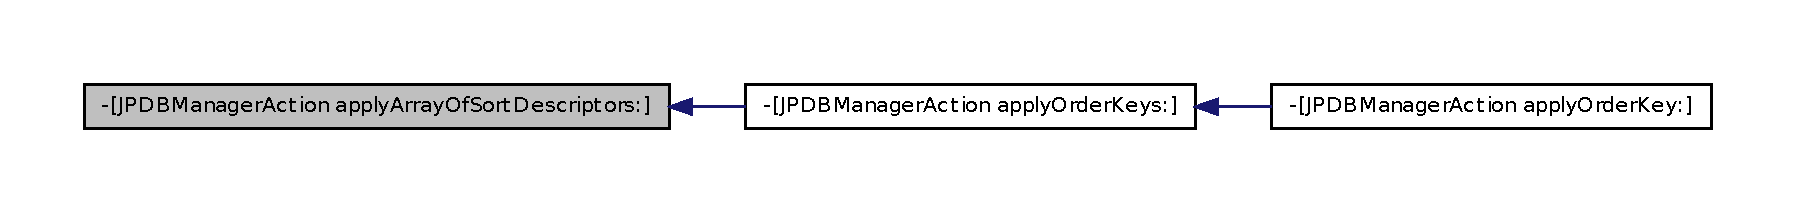
\includegraphics[width=400pt]{interface_j_p_d_b_manager_action_ac7b38fbbab436a50344de7e5c61238b8_icgraph}
\end{center}
\end{figure}


\hypertarget{interface_j_p_d_b_manager_action_aab038bf441025fe2d6615a49d67d6477}{
\index{JPDBManagerAction@{JPDBManagerAction}!applyOrderKeys:@{applyOrderKeys:}}
\index{applyOrderKeys:@{applyOrderKeys:}!JPDBManagerAction@{JPDBManagerAction}}
\subsubsection[{applyOrderKeys:}]{\setlength{\rightskip}{0pt plus 5cm}-\/ (id) applyOrderKeys: 
\begin{DoxyParamCaption}
\item[{dummy(id)}]{listOfKeys}
\item[{,}]{NS\_\-REQUIRES\_\-NIL\_\-TERMINATION}
\end{DoxyParamCaption}
}}
\label{interface_j_p_d_b_manager_action_aab038bf441025fe2d6615a49d67d6477}


Set the Key attributes to sort the result of this acion. 


\begin{DoxyParams}{Parameters}
{\em listOfKeys} & Accept one or more Key Attributes to sort the result. Doesn't forget to terminate the list with an 'nil' token. \\
\hline
\end{DoxyParams}
\begin{DoxyReturn}{Returns}
Return itself. 
\end{DoxyReturn}

\begin{DoxyExceptions}{Exceptions}
{\em An} & \hyperlink{errors_JPDBManagerActionException}{JPDBManagerActionException} exception if the \hyperlink{interface_j_p_d_b_manager_action_a705cfdcdfd4ff48deff4ba42928412b9}{entity} property isn't defined. See \hyperlink{errors}{Handling Errors} for more informations. \\
\hline
\end{DoxyExceptions}


Here is the call graph for this function:
\nopagebreak
\begin{figure}[H]
\begin{center}
\leavevmode
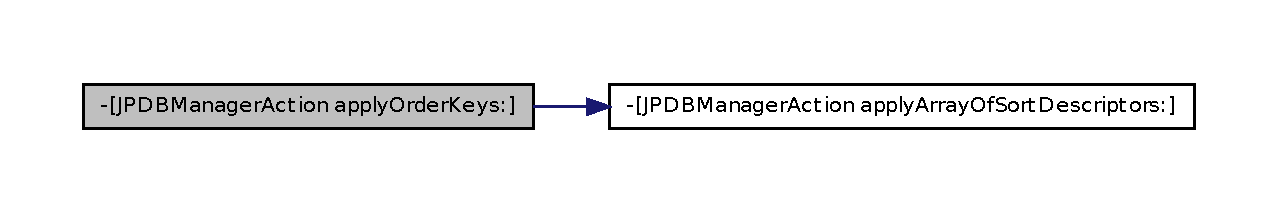
\includegraphics[width=400pt]{interface_j_p_d_b_manager_action_aab038bf441025fe2d6615a49d67d6477_cgraph}
\end{center}
\end{figure}




Here is the caller graph for this function:
\nopagebreak
\begin{figure}[H]
\begin{center}
\leavevmode
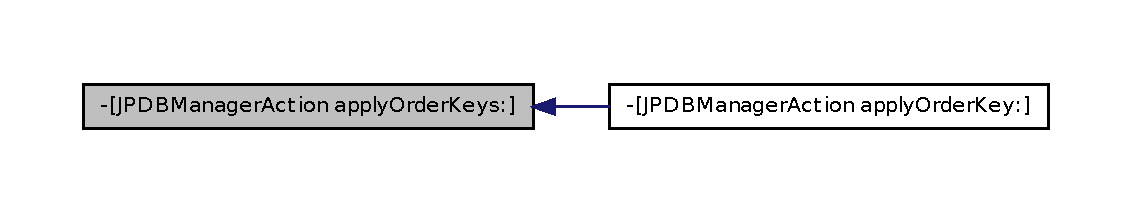
\includegraphics[width=400pt]{interface_j_p_d_b_manager_action_aab038bf441025fe2d6615a49d67d6477_icgraph}
\end{center}
\end{figure}


\hypertarget{interface_j_p_d_b_manager_action_a432c1012382e6baa4c76c051a524881e}{
\index{JPDBManagerAction@{JPDBManagerAction}!applyOrderKey:@{applyOrderKey:}}
\index{applyOrderKey:@{applyOrderKey:}!JPDBManagerAction@{JPDBManagerAction}}
\subsubsection[{applyOrderKey:}]{\setlength{\rightskip}{0pt plus 5cm}-\/ (id) applyOrderKey: 
\begin{DoxyParamCaption}
\item[{dummy(id)}]{anKey}
\end{DoxyParamCaption}
}}
\label{interface_j_p_d_b_manager_action_a432c1012382e6baa4c76c051a524881e}


Set the Key attribute to sort the result of this acion. 


\begin{DoxyParams}{Parameters}
{\em anKey} & An Key Attribute to sort the result. \\
\hline
\end{DoxyParams}
\begin{DoxyReturn}{Returns}
Return itself. 
\end{DoxyReturn}

\begin{DoxyExceptions}{Exceptions}
{\em An} & \hyperlink{errors_JPDBManagerActionException}{JPDBManagerActionException} exception if the \hyperlink{interface_j_p_d_b_manager_action_a705cfdcdfd4ff48deff4ba42928412b9}{entity} property isn't defined. See \hyperlink{errors}{Handling Errors} for more informations. \\
\hline
\end{DoxyExceptions}


Here is the call graph for this function:
\nopagebreak
\begin{figure}[H]
\begin{center}
\leavevmode
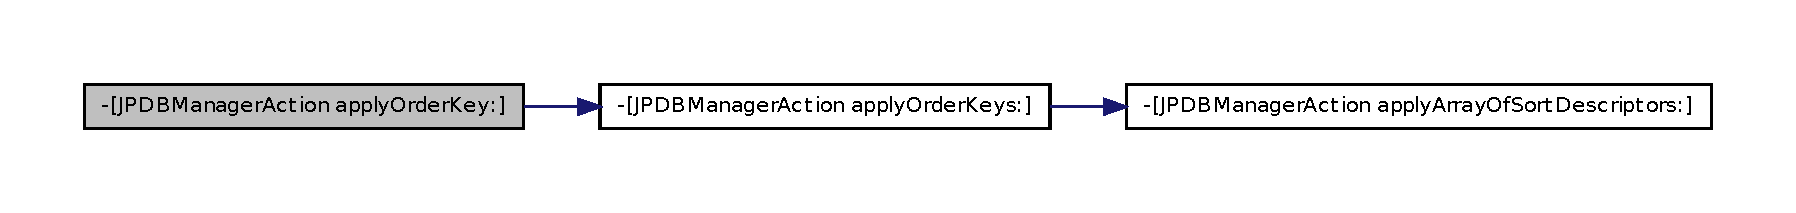
\includegraphics[width=400pt]{interface_j_p_d_b_manager_action_a432c1012382e6baa4c76c051a524881e_cgraph}
\end{center}
\end{figure}


\hypertarget{interface_j_p_d_b_manager_action_a2ed39b1660529638ea1596cfea71580d}{
\index{JPDBManagerAction@{JPDBManagerAction}!addOrderKey:@{addOrderKey:}}
\index{addOrderKey:@{addOrderKey:}!JPDBManagerAction@{JPDBManagerAction}}
\subsubsection[{addOrderKey:}]{\setlength{\rightskip}{0pt plus 5cm}-\/ (id) addOrderKey: 
\begin{DoxyParamCaption}
\item[{dummy(id)}]{anKey}
\end{DoxyParamCaption}
}}
\label{interface_j_p_d_b_manager_action_a2ed39b1660529638ea1596cfea71580d}


Add a new Key attribute to sort the result of this action. 


\begin{DoxyParams}{Parameters}
{\em anKey} & An Key Attribute to sort the result. \\
\hline
\end{DoxyParams}
\begin{DoxyReturn}{Returns}
Return itself. 
\end{DoxyReturn}

\begin{DoxyExceptions}{Exceptions}
{\em An} & \hyperlink{errors_JPDBManagerActionException}{JPDBManagerActionException} exception if the \hyperlink{interface_j_p_d_b_manager_action_a705cfdcdfd4ff48deff4ba42928412b9}{entity} property isn't defined. See \hyperlink{errors}{Handling Errors} for more informations. \\
\hline
\end{DoxyExceptions}
\hypertarget{interface_j_p_d_b_manager_action_a5ca5bdf039427760eb017fd51575d0e2}{
\index{JPDBManagerAction@{JPDBManagerAction}!removeOrderKey:@{removeOrderKey:}}
\index{removeOrderKey:@{removeOrderKey:}!JPDBManagerAction@{JPDBManagerAction}}
\subsubsection[{removeOrderKey:}]{\setlength{\rightskip}{0pt plus 5cm}-\/ (void) removeOrderKey: 
\begin{DoxyParamCaption}
\item[{dummy(id)}]{anKey}
\end{DoxyParamCaption}
}}
\label{interface_j_p_d_b_manager_action_a5ca5bdf039427760eb017fd51575d0e2}


Remove an Key attribute from the sorter list. 


\begin{DoxyParams}{Parameters}
{\em anKey} & An Key Attribute to remove. \\
\hline
\end{DoxyParams}
\hypertarget{interface_j_p_d_b_manager_action_a367267b639633531a6e44c6b7857cfd0}{
\index{JPDBManagerAction@{JPDBManagerAction}!queryAllDataFromEntity:@{queryAllDataFromEntity:}}
\index{queryAllDataFromEntity:@{queryAllDataFromEntity:}!JPDBManagerAction@{JPDBManagerAction}}
\subsubsection[{queryAllDataFromEntity:}]{\setlength{\rightskip}{0pt plus 5cm}-\/ (id) queryAllDataFromEntity: 
\begin{DoxyParamCaption}
\item[{dummy(NSString$\ast$)}]{anEntityName}
\end{DoxyParamCaption}
}}
\label{interface_j_p_d_b_manager_action_a367267b639633531a6e44c6b7857cfd0}


Query all data of the specified Entity. 


\begin{DoxyParams}{Parameters}
{\em anEntityName} & The Entity Name. \\
\hline
\end{DoxyParams}
\begin{DoxyReturn}{Returns}
One unordered collection with queried data Objects. The Class of this collection is setted by \#returnQueryAsArray property. 
\end{DoxyReturn}


Here is the call graph for this function:
\nopagebreak
\begin{figure}[H]
\begin{center}
\leavevmode
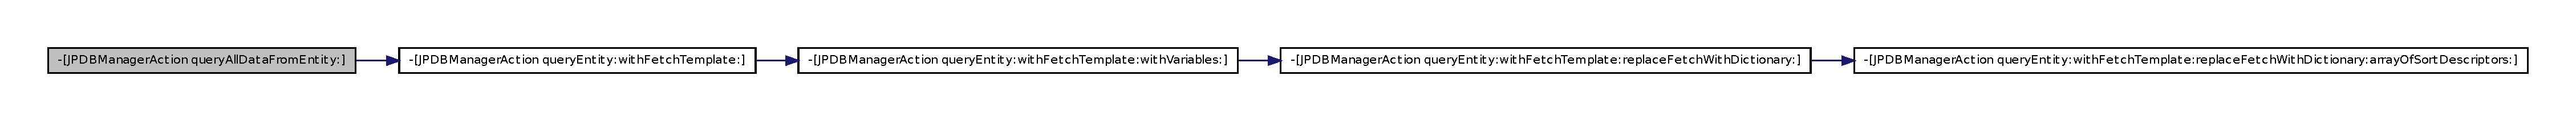
\includegraphics[width=400pt]{interface_j_p_d_b_manager_action_a367267b639633531a6e44c6b7857cfd0_cgraph}
\end{center}
\end{figure}


\hypertarget{interface_j_p_d_b_manager_action_a41146d672b6282be3eb7ef37dffe17d0}{
\index{JPDBManagerAction@{JPDBManagerAction}!queryAllDataFromEntity:orderWithKey:@{queryAllDataFromEntity:orderWithKey:}}
\index{queryAllDataFromEntity:orderWithKey:@{queryAllDataFromEntity:orderWithKey:}!JPDBManagerAction@{JPDBManagerAction}}
\subsubsection[{queryAllDataFromEntity:orderWithKey:}]{\setlength{\rightskip}{0pt plus 5cm}-\/ (id) queryAllDataFromEntity: 
\begin{DoxyParamCaption}
\item[{dummy(NSString$\ast$)}]{anEntityName}
\item[{orderWithKey:(id)}]{anKey}
\end{DoxyParamCaption}
}}
\label{interface_j_p_d_b_manager_action_a41146d672b6282be3eb7ef37dffe17d0}


Query all data of the specified Entity. 

The \#defaultOrderIsAscending property determines if is an Ascending or Descending order. 
\begin{DoxyParams}{Parameters}
{\em anEntityName} & The Entity Name. \\
\hline
{\em anKey} & One Key attribute to sort the result. \\
\hline
\end{DoxyParams}
\begin{DoxyReturn}{Returns}
One unordered collection with queried data Objects. The Class of this collection is setted by \#returnQueryAsArray property. 
\end{DoxyReturn}


Here is the call graph for this function:
\nopagebreak
\begin{figure}[H]
\begin{center}
\leavevmode
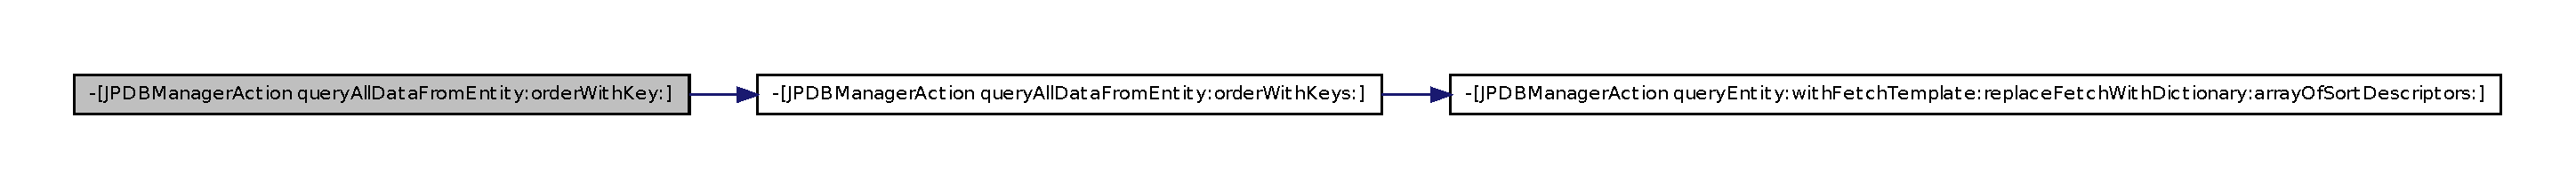
\includegraphics[width=400pt]{interface_j_p_d_b_manager_action_a41146d672b6282be3eb7ef37dffe17d0_cgraph}
\end{center}
\end{figure}


\hypertarget{interface_j_p_d_b_manager_action_ad26a0af6246a53d8497178371308e28d}{
\index{JPDBManagerAction@{JPDBManagerAction}!queryAllDataFromEntity:orderWithKeys:@{queryAllDataFromEntity:orderWithKeys:}}
\index{queryAllDataFromEntity:orderWithKeys:@{queryAllDataFromEntity:orderWithKeys:}!JPDBManagerAction@{JPDBManagerAction}}
\subsubsection[{queryAllDataFromEntity:orderWithKeys:}]{\setlength{\rightskip}{0pt plus 5cm}-\/ (id) queryAllDataFromEntity: 
\begin{DoxyParamCaption}
\item[{dummy(NSString$\ast$)}]{anEntityName}
\item[{orderWithKeys:(id)}]{listOfKeys}
\item[{,}]{NS\_\-REQUIRES\_\-NIL\_\-TERMINATION}
\end{DoxyParamCaption}
}}
\label{interface_j_p_d_b_manager_action_ad26a0af6246a53d8497178371308e28d}


Query all data of the specified Entity. 


\begin{DoxyParams}{Parameters}
{\em anEntityName} & The Entity Name. \\
\hline
{\em listOfKeys} & Accept one or more Key Attributes to sort the result. Doesn't forget to terminate the list with an 'nil' token. \\
\hline
\end{DoxyParams}
\begin{DoxyReturn}{Returns}
One unordered collection with queried data Objects. The Class of this collection is setted by \#returnQueryAsArray property. 
\end{DoxyReturn}


Here is the call graph for this function:
\nopagebreak
\begin{figure}[H]
\begin{center}
\leavevmode
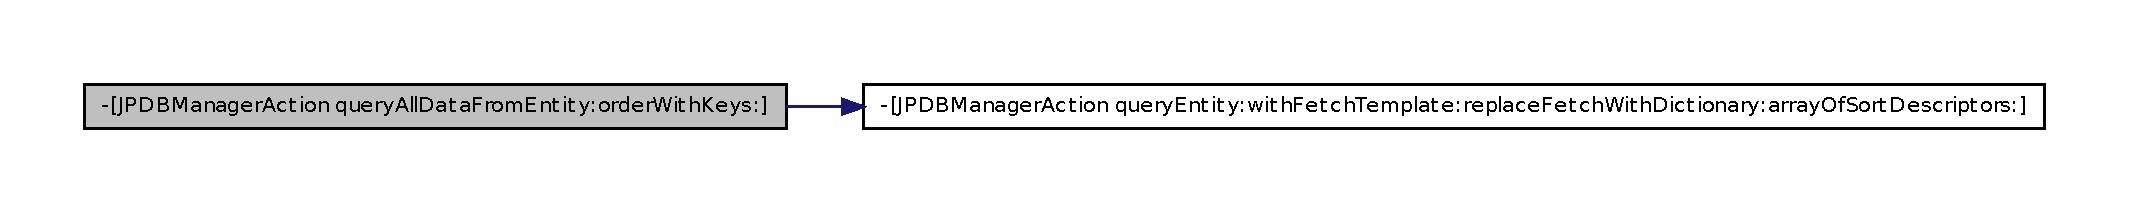
\includegraphics[width=400pt]{interface_j_p_d_b_manager_action_ad26a0af6246a53d8497178371308e28d_cgraph}
\end{center}
\end{figure}




Here is the caller graph for this function:
\nopagebreak
\begin{figure}[H]
\begin{center}
\leavevmode
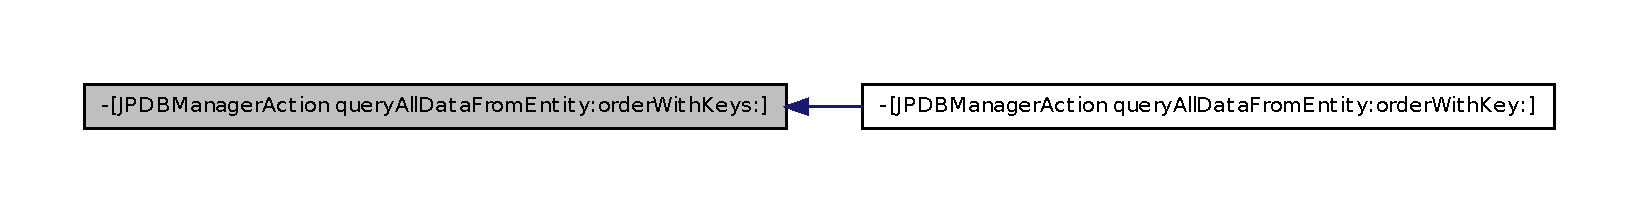
\includegraphics[width=400pt]{interface_j_p_d_b_manager_action_ad26a0af6246a53d8497178371308e28d_icgraph}
\end{center}
\end{figure}


\hypertarget{interface_j_p_d_b_manager_action_a37853bbac86c15f62981187bd9d7bcfc}{
\index{JPDBManagerAction@{JPDBManagerAction}!queryEntity:withFetchTemplate:@{queryEntity:withFetchTemplate:}}
\index{queryEntity:withFetchTemplate:@{queryEntity:withFetchTemplate:}!JPDBManagerAction@{JPDBManagerAction}}
\subsubsection[{queryEntity:withFetchTemplate:}]{\setlength{\rightskip}{0pt plus 5cm}-\/ (id) queryEntity: 
\begin{DoxyParamCaption}
\item[{dummy(NSString$\ast$)}]{anEntityName}
\item[{withFetchTemplate:(NSString$\ast$)}]{anFetchName}
\end{DoxyParamCaption}
}}
\label{interface_j_p_d_b_manager_action_a37853bbac86c15f62981187bd9d7bcfc}


Query specified Entity using one specified Fetch Template name. 


\begin{DoxyParams}{Parameters}
{\em anEntityName} & The Entity Name. \\
\hline
{\em anFetchName} & An Fetch Template to perform the query. \\
\hline
\end{DoxyParams}
\begin{DoxyReturn}{Returns}
One unordered collection with queried data Objects. The Class of this collection is setted by \#returnQueryAsArray property. 
\end{DoxyReturn}


Here is the call graph for this function:
\nopagebreak
\begin{figure}[H]
\begin{center}
\leavevmode
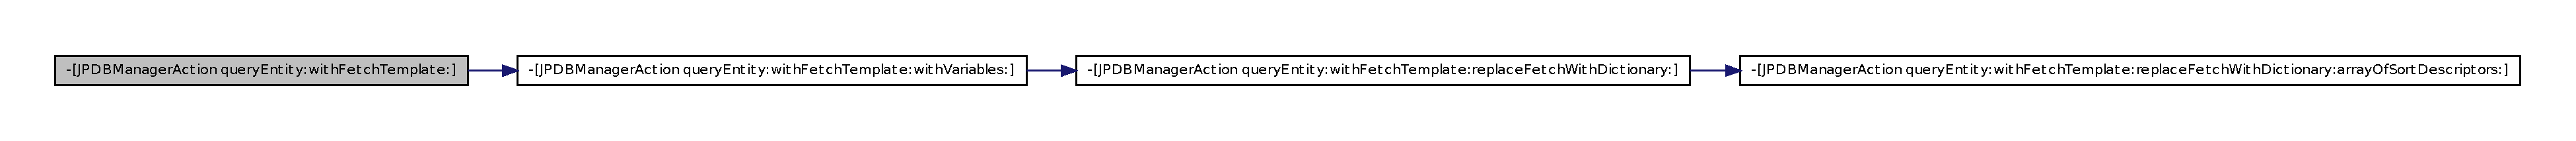
\includegraphics[width=400pt]{interface_j_p_d_b_manager_action_a37853bbac86c15f62981187bd9d7bcfc_cgraph}
\end{center}
\end{figure}




Here is the caller graph for this function:
\nopagebreak
\begin{figure}[H]
\begin{center}
\leavevmode
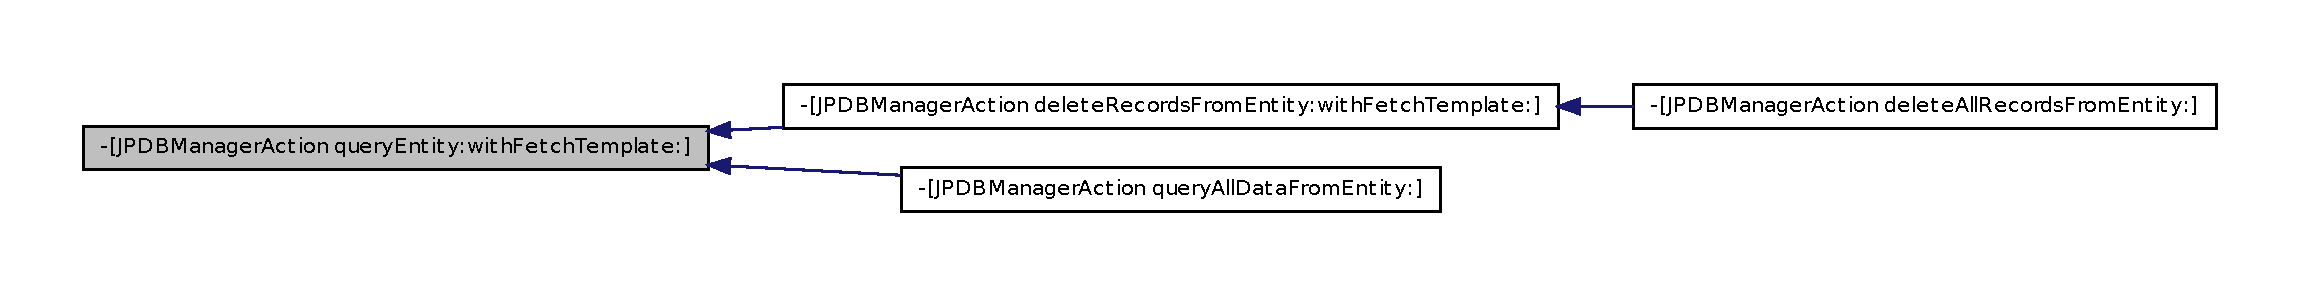
\includegraphics[width=400pt]{interface_j_p_d_b_manager_action_a37853bbac86c15f62981187bd9d7bcfc_icgraph}
\end{center}
\end{figure}


\hypertarget{interface_j_p_d_b_manager_action_aa857b7593c614e34728ba1c346774e47}{
\index{JPDBManagerAction@{JPDBManagerAction}!queryEntity:withFetchTemplate:orderWithKey:@{queryEntity:withFetchTemplate:orderWithKey:}}
\index{queryEntity:withFetchTemplate:orderWithKey:@{queryEntity:withFetchTemplate:orderWithKey:}!JPDBManagerAction@{JPDBManagerAction}}
\subsubsection[{queryEntity:withFetchTemplate:orderWithKey:}]{\setlength{\rightskip}{0pt plus 5cm}-\/ (id) queryEntity: 
\begin{DoxyParamCaption}
\item[{dummy(NSString$\ast$)}]{anEntityName}
\item[{withFetchTemplate:(NSString$\ast$)}]{anFetchName}
\item[{orderWithKey:(id)}]{anKey}
\end{DoxyParamCaption}
}}
\label{interface_j_p_d_b_manager_action_aa857b7593c614e34728ba1c346774e47}


Query specified Entity using one specified Fetch Template name. 


\begin{DoxyParams}{Parameters}
{\em anEntityName} & The Entity Name. \\
\hline
{\em anFetchName} & An Fetch Template to perform the query. \\
\hline
{\em anKey} & One Key attribute to sort the result. \\
\hline
\end{DoxyParams}
\begin{DoxyReturn}{Returns}
One unordered collection with queried data Objects. The Class of this collection is setted by \#returnQueryAsArray property. 
\end{DoxyReturn}


Here is the call graph for this function:
\nopagebreak
\begin{figure}[H]
\begin{center}
\leavevmode
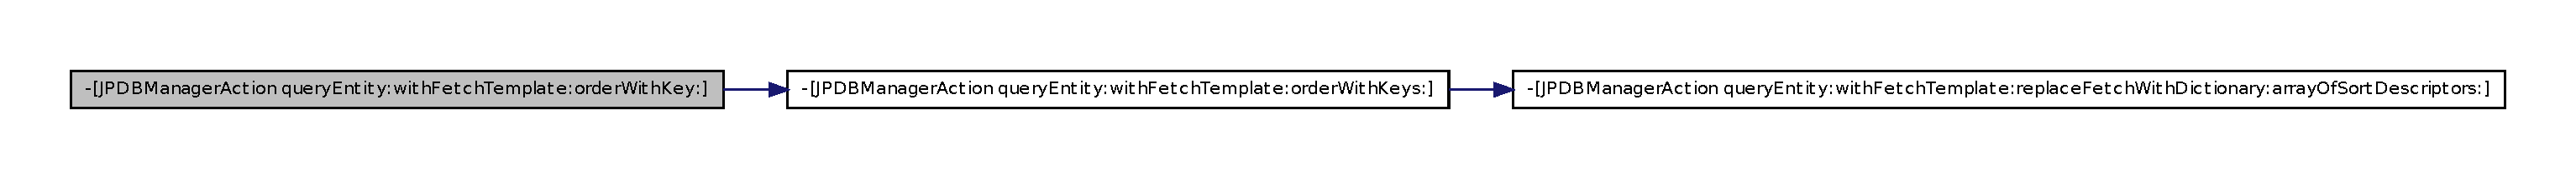
\includegraphics[width=400pt]{interface_j_p_d_b_manager_action_aa857b7593c614e34728ba1c346774e47_cgraph}
\end{center}
\end{figure}


\hypertarget{interface_j_p_d_b_manager_action_ac9cc8404e73e1cb38ce0cc50cbac3ecd}{
\index{JPDBManagerAction@{JPDBManagerAction}!queryEntity:withFetchTemplate:orderWithKeys:@{queryEntity:withFetchTemplate:orderWithKeys:}}
\index{queryEntity:withFetchTemplate:orderWithKeys:@{queryEntity:withFetchTemplate:orderWithKeys:}!JPDBManagerAction@{JPDBManagerAction}}
\subsubsection[{queryEntity:withFetchTemplate:orderWithKeys:}]{\setlength{\rightskip}{0pt plus 5cm}-\/ (id) queryEntity: 
\begin{DoxyParamCaption}
\item[{dummy(NSString$\ast$)}]{anEntityName}
\item[{withFetchTemplate:(NSString$\ast$)}]{anFetchName}
\item[{orderWithKeys:(id)}]{listOfKeys}
\item[{,}]{NS\_\-REQUIRES\_\-NIL\_\-TERMINATION}
\end{DoxyParamCaption}
}}
\label{interface_j_p_d_b_manager_action_ac9cc8404e73e1cb38ce0cc50cbac3ecd}


Query specified Entity using one specified Fetch Template name. 


\begin{DoxyParams}{Parameters}
{\em anEntityName} & The Entity Name. \\
\hline
{\em anFetchName} & An Fetch Template to perform the query. \\
\hline
{\em listOfKeys} & Accept one or more Key Attributes to sort the result. Doesn't forget to terminate the list with an 'nil' token. \\
\hline
\end{DoxyParams}
\begin{DoxyReturn}{Returns}
One unordered collection with queried data Objects. The Class of this collection is setted by \#returnQueryAsArray property. 
\end{DoxyReturn}


Here is the call graph for this function:
\nopagebreak
\begin{figure}[H]
\begin{center}
\leavevmode
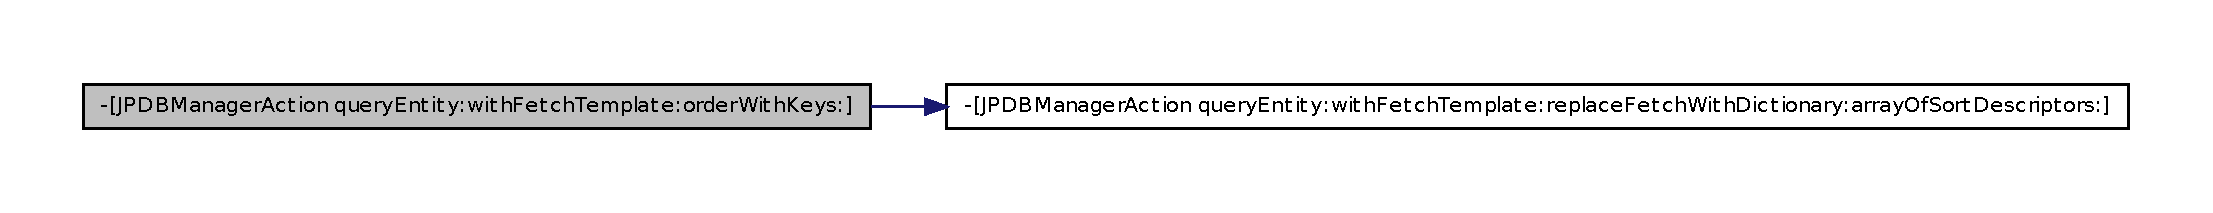
\includegraphics[width=400pt]{interface_j_p_d_b_manager_action_ac9cc8404e73e1cb38ce0cc50cbac3ecd_cgraph}
\end{center}
\end{figure}




Here is the caller graph for this function:
\nopagebreak
\begin{figure}[H]
\begin{center}
\leavevmode
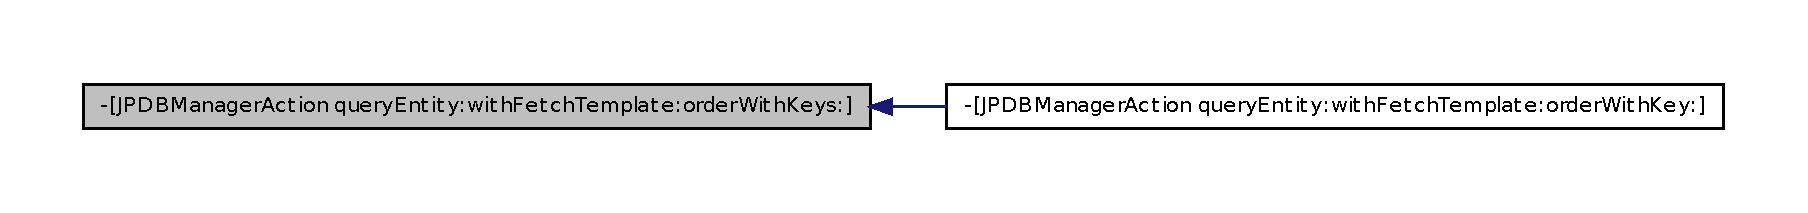
\includegraphics[width=400pt]{interface_j_p_d_b_manager_action_ac9cc8404e73e1cb38ce0cc50cbac3ecd_icgraph}
\end{center}
\end{figure}


\hypertarget{interface_j_p_d_b_manager_action_aac56b1fa8bf99688b4ea5f117036eff0}{
\index{JPDBManagerAction@{JPDBManagerAction}!queryEntity:withFetchTemplate:withVariables:@{queryEntity:withFetchTemplate:withVariables:}}
\index{queryEntity:withFetchTemplate:withVariables:@{queryEntity:withFetchTemplate:withVariables:}!JPDBManagerAction@{JPDBManagerAction}}
\subsubsection[{queryEntity:withFetchTemplate:withVariables:}]{\setlength{\rightskip}{0pt plus 5cm}-\/ (id) queryEntity: 
\begin{DoxyParamCaption}
\item[{dummy(NSString$\ast$)}]{anEntityName}
\item[{withFetchTemplate:(NSString$\ast$)}]{anFetchName}
\item[{withVariables:(id)}]{variableList}
\item[{,}]{NS\_\-REQUIRES\_\-NIL\_\-TERMINATION}
\end{DoxyParamCaption}
}}
\label{interface_j_p_d_b_manager_action_aac56b1fa8bf99688b4ea5f117036eff0}


Query specified Entity using one specified Fetch Template name. 


\begin{DoxyParams}{Parameters}
{\em anEntityName} & The Entity Name. \\
\hline
{\em anFetchName} & An Fetch Template to perform the query. \\
\hline
{\em variableList} & Keys and Values to replace on the pre formatted Fetch Template.\par
 {\bfseries Example:}\par
 
\begin{DoxyCode}
 [manager queryEntity:@"Entity" 
   withFetchTemplate:@"FetchAll"
       withVariables:@"value1", @"key1", @"value2", @"key2", nil];
\end{DoxyCode}
 \\
\hline
\end{DoxyParams}
\begin{DoxyReturn}{Returns}
One unordered collection with queried data Objects. The Class of this collection is setted by \#returnQueryAsArray property. 
\end{DoxyReturn}


Here is the call graph for this function:
\nopagebreak
\begin{figure}[H]
\begin{center}
\leavevmode
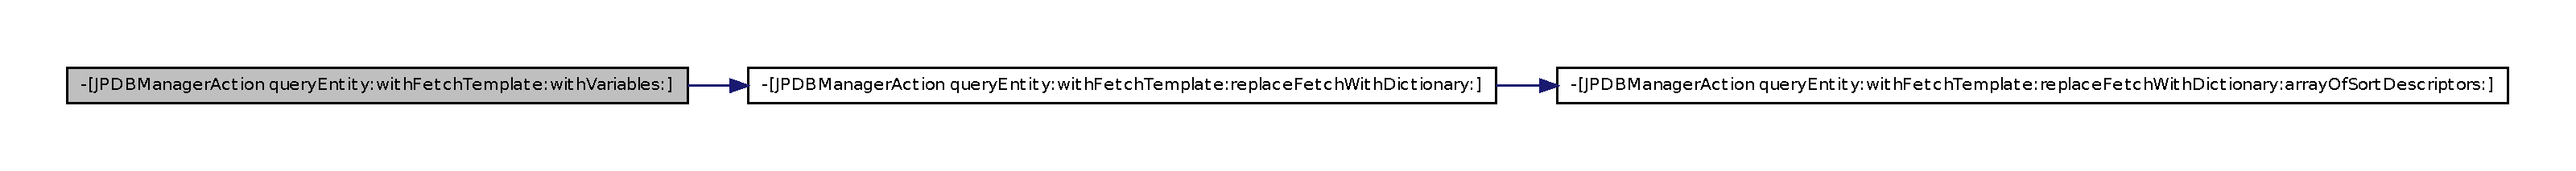
\includegraphics[width=400pt]{interface_j_p_d_b_manager_action_aac56b1fa8bf99688b4ea5f117036eff0_cgraph}
\end{center}
\end{figure}




Here is the caller graph for this function:
\nopagebreak
\begin{figure}[H]
\begin{center}
\leavevmode
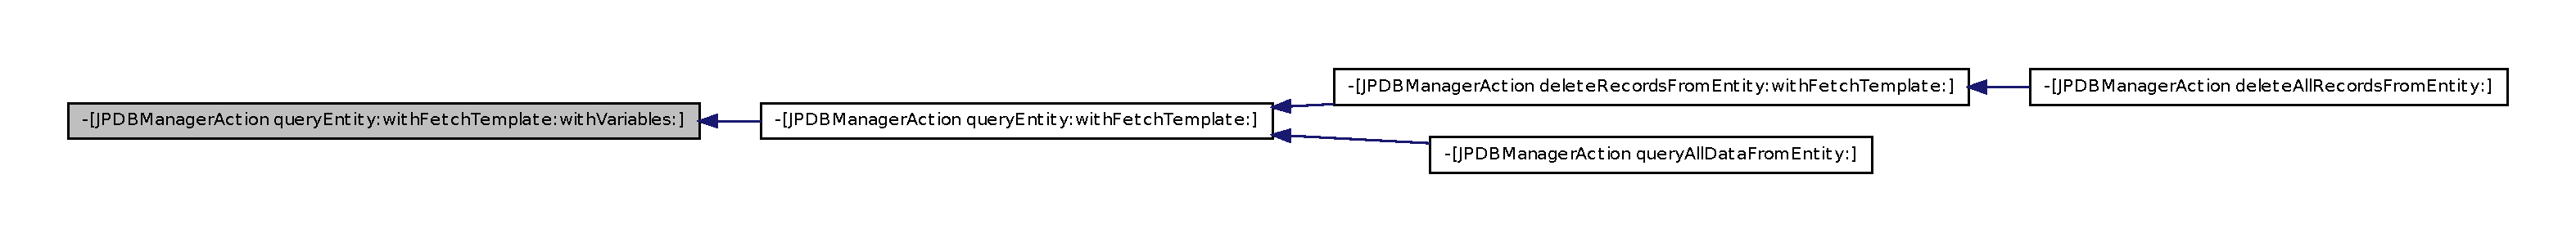
\includegraphics[width=400pt]{interface_j_p_d_b_manager_action_aac56b1fa8bf99688b4ea5f117036eff0_icgraph}
\end{center}
\end{figure}


\hypertarget{interface_j_p_d_b_manager_action_a3044583007eb7aa00185a5da222acc40}{
\index{JPDBManagerAction@{JPDBManagerAction}!queryEntity:withFetchTemplate:orderWithKey:withVariables:@{queryEntity:withFetchTemplate:orderWithKey:withVariables:}}
\index{queryEntity:withFetchTemplate:orderWithKey:withVariables:@{queryEntity:withFetchTemplate:orderWithKey:withVariables:}!JPDBManagerAction@{JPDBManagerAction}}
\subsubsection[{queryEntity:withFetchTemplate:orderWithKey:withVariables:}]{\setlength{\rightskip}{0pt plus 5cm}-\/ (id) queryEntity: 
\begin{DoxyParamCaption}
\item[{dummy(NSString$\ast$)}]{anEntityName}
\item[{withFetchTemplate:(NSString$\ast$)}]{anFetchName}
\item[{orderWithKey:(id)}]{anKey}
\item[{withVariables:(id)}]{variableList}
\item[{,}]{NS\_\-REQUIRES\_\-NIL\_\-TERMINATION}
\end{DoxyParamCaption}
}}
\label{interface_j_p_d_b_manager_action_a3044583007eb7aa00185a5da222acc40}


Query specified Entity using one specified Fetch Template name. 


\begin{DoxyParams}{Parameters}
{\em anEntityName} & The Entity Name. \\
\hline
{\em anFetchName} & An Fetch Template to perform the query. \\
\hline
{\em anKey} & One Key attribute to sort the result. \\
\hline
{\em variableList} & Keys and Values to replace on the pre formatted Fetch Template.\par
 {\bfseries Example:}\par
 
\begin{DoxyCode}
 [manager queryEntity:@"Entity" 
   withFetchTemplate:@"FetchAll"
        orderWithKey:@"id" 
       withVariables:@"value1", @"key1", @"value2", @"key2", nil];
\end{DoxyCode}
 \\
\hline
\end{DoxyParams}
\begin{DoxyReturn}{Returns}
One unordered collection with queried data Objects. The Class of this collection is setted by \#returnQueryAsArray property. 
\end{DoxyReturn}


Here is the call graph for this function:
\nopagebreak
\begin{figure}[H]
\begin{center}
\leavevmode
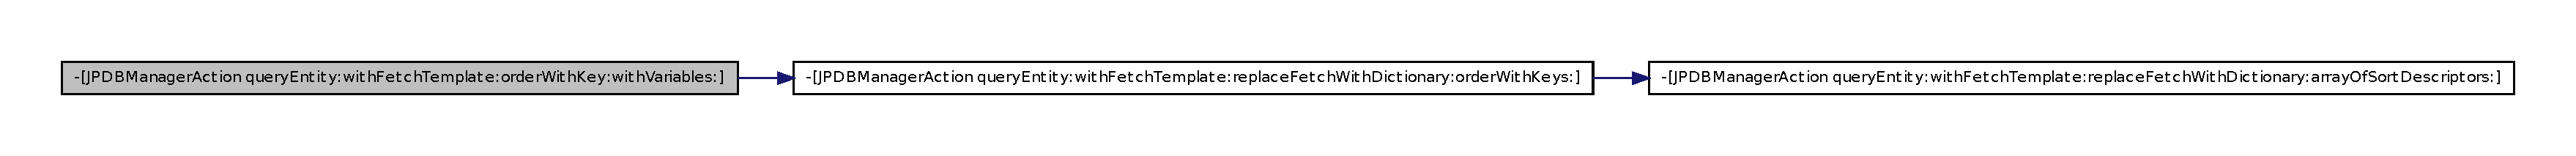
\includegraphics[width=400pt]{interface_j_p_d_b_manager_action_a3044583007eb7aa00185a5da222acc40_cgraph}
\end{center}
\end{figure}


\hypertarget{interface_j_p_d_b_manager_action_ae32ca03d7ce37116f5c9e292e368bf8f}{
\index{JPDBManagerAction@{JPDBManagerAction}!queryEntity:withFetchTemplate:replaceFetchWithDictionary:@{queryEntity:withFetchTemplate:replaceFetchWithDictionary:}}
\index{queryEntity:withFetchTemplate:replaceFetchWithDictionary:@{queryEntity:withFetchTemplate:replaceFetchWithDictionary:}!JPDBManagerAction@{JPDBManagerAction}}
\subsubsection[{queryEntity:withFetchTemplate:replaceFetchWithDictionary:}]{\setlength{\rightskip}{0pt plus 5cm}-\/ (id) queryEntity: 
\begin{DoxyParamCaption}
\item[{dummy(NSString$\ast$)}]{anEntityName}
\item[{withFetchTemplate:(NSString$\ast$)}]{anFetchName}
\item[{replaceFetchWithDictionary:(NSDictionary$\ast$)}]{variablesListAndValues}
\end{DoxyParamCaption}
}}
\label{interface_j_p_d_b_manager_action_ae32ca03d7ce37116f5c9e292e368bf8f}


Query specified Entity using one specified Fetch Template name. 


\begin{DoxyParams}{Parameters}
{\em anEntityName} & The Entity Name. \\
\hline
{\em anFetchName} & An Fetch Template to perform the query. \\
\hline
{\em variablesListAndValues} & An Dictionary with Keys and Values to replace on the pre formatted Fetch Template. \\
\hline
\end{DoxyParams}
\begin{DoxyReturn}{Returns}
One unordered collection with queried data Objects. The Class of this collection is setted by \#returnQueryAsArray property. 
\end{DoxyReturn}


Here is the call graph for this function:
\nopagebreak
\begin{figure}[H]
\begin{center}
\leavevmode
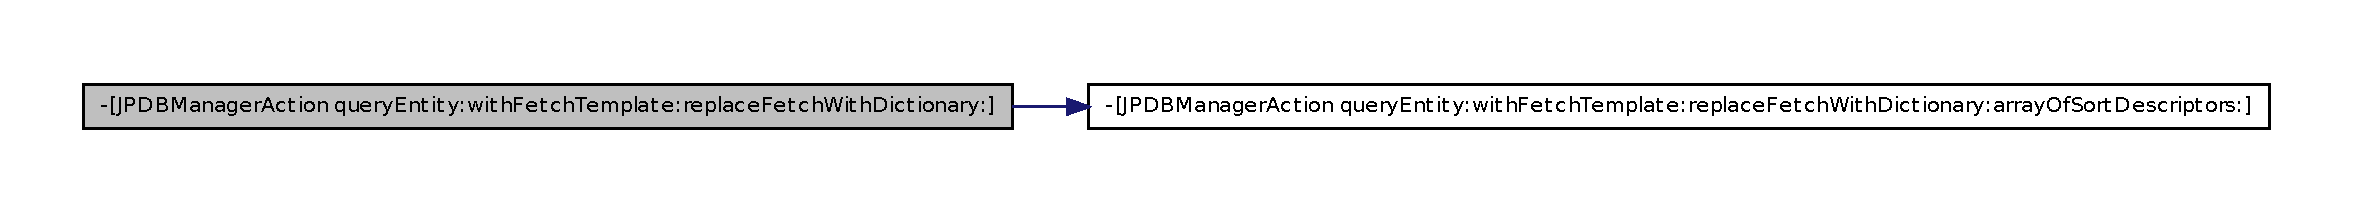
\includegraphics[width=400pt]{interface_j_p_d_b_manager_action_ae32ca03d7ce37116f5c9e292e368bf8f_cgraph}
\end{center}
\end{figure}




Here is the caller graph for this function:
\nopagebreak
\begin{figure}[H]
\begin{center}
\leavevmode
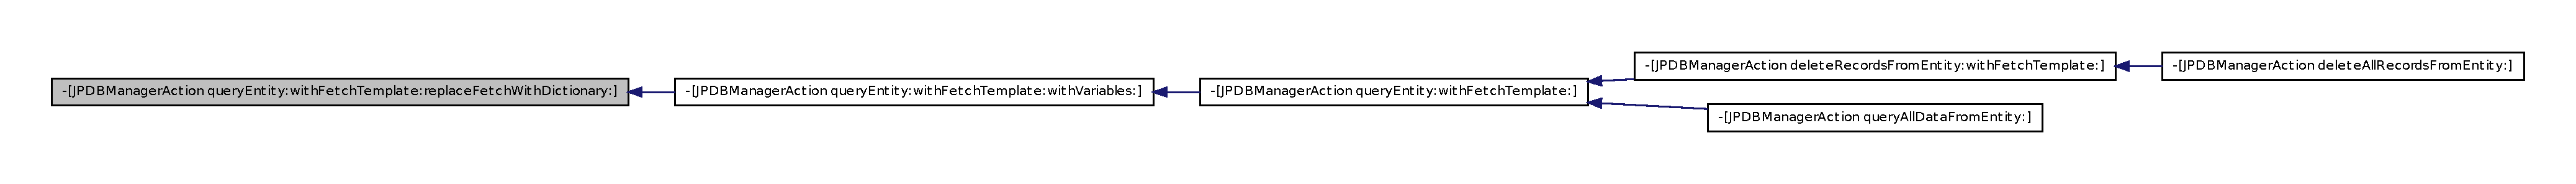
\includegraphics[width=400pt]{interface_j_p_d_b_manager_action_ae32ca03d7ce37116f5c9e292e368bf8f_icgraph}
\end{center}
\end{figure}


\hypertarget{interface_j_p_d_b_manager_action_aef6b587a0260a962b3ba9946d5590997}{
\index{JPDBManagerAction@{JPDBManagerAction}!queryEntity:withFetchTemplate:replaceFetchWithDictionary:orderWithKey:@{queryEntity:withFetchTemplate:replaceFetchWithDictionary:orderWithKey:}}
\index{queryEntity:withFetchTemplate:replaceFetchWithDictionary:orderWithKey:@{queryEntity:withFetchTemplate:replaceFetchWithDictionary:orderWithKey:}!JPDBManagerAction@{JPDBManagerAction}}
\subsubsection[{queryEntity:withFetchTemplate:replaceFetchWithDictionary:orderWithKey:}]{\setlength{\rightskip}{0pt plus 5cm}-\/ (id) queryEntity: 
\begin{DoxyParamCaption}
\item[{dummy(NSString$\ast$)}]{anEntityName}
\item[{withFetchTemplate:(NSString$\ast$)}]{anFetchName}
\item[{replaceFetchWithDictionary:(NSDictionary$\ast$)}]{variablesListAndValues}
\item[{orderWithKey:(id)}]{anKey}
\end{DoxyParamCaption}
}}
\label{interface_j_p_d_b_manager_action_aef6b587a0260a962b3ba9946d5590997}


Query specified Entity using one specified Fetch Template name. 


\begin{DoxyParams}{Parameters}
{\em anEntityName} & The Entity Name. \\
\hline
{\em anFetchName} & An Fetch Template to perform the query. \\
\hline
{\em variablesListAndValues} & An Dictionary with Keys and Values to replace on the pre formatted Fetch Template. \\
\hline
{\em anKey} & One Key attribute to sort the result. \\
\hline
\end{DoxyParams}
\begin{DoxyReturn}{Returns}
One unordered collection with queried data Objects. The Class of this collection is setted by \#returnQueryAsArray property. 
\end{DoxyReturn}


Here is the call graph for this function:
\nopagebreak
\begin{figure}[H]
\begin{center}
\leavevmode
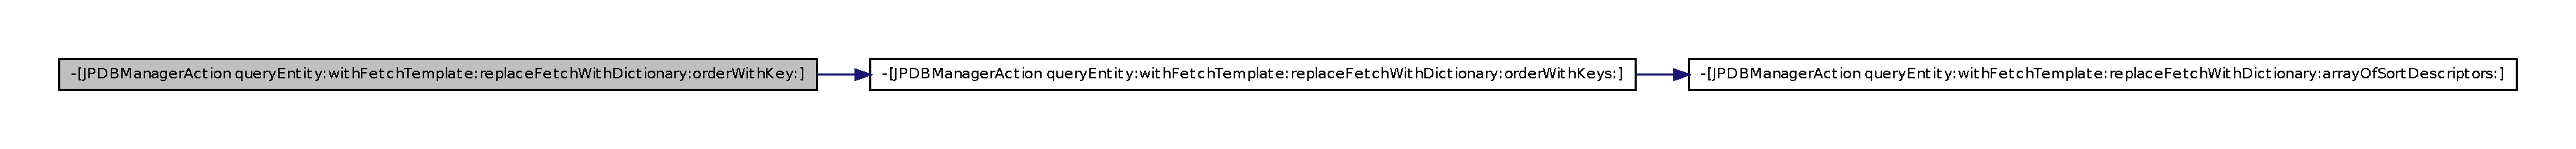
\includegraphics[width=400pt]{interface_j_p_d_b_manager_action_aef6b587a0260a962b3ba9946d5590997_cgraph}
\end{center}
\end{figure}


\hypertarget{interface_j_p_d_b_manager_action_ac04b76b32d39ae9b412f99b3ac620a86}{
\index{JPDBManagerAction@{JPDBManagerAction}!queryEntity:withFetchTemplate:replaceFetchWithDictionary:orderWithKeys:@{queryEntity:withFetchTemplate:replaceFetchWithDictionary:orderWithKeys:}}
\index{queryEntity:withFetchTemplate:replaceFetchWithDictionary:orderWithKeys:@{queryEntity:withFetchTemplate:replaceFetchWithDictionary:orderWithKeys:}!JPDBManagerAction@{JPDBManagerAction}}
\subsubsection[{queryEntity:withFetchTemplate:replaceFetchWithDictionary:orderWithKeys:}]{\setlength{\rightskip}{0pt plus 5cm}-\/ (id) queryEntity: 
\begin{DoxyParamCaption}
\item[{dummy(NSString$\ast$)}]{anEntityName}
\item[{withFetchTemplate:(NSString$\ast$)}]{anFetchName}
\item[{replaceFetchWithDictionary:(NSDictionary$\ast$)}]{variablesListAndValues}
\item[{orderWithKeys:(id)}]{listOfKeys}
\item[{,}]{NS\_\-REQUIRES\_\-NIL\_\-TERMINATION}
\end{DoxyParamCaption}
}}
\label{interface_j_p_d_b_manager_action_ac04b76b32d39ae9b412f99b3ac620a86}


Query specified Entity using one specified Fetch Template name. 


\begin{DoxyParams}{Parameters}
{\em anEntityName} & The Entity Name. \\
\hline
{\em anFetchName} & An Fetch Template to perform the query. \\
\hline
{\em variablesListAndValues} & An Dictionary with Keys and Values to replace on the pre formatted Fetch Template. \\
\hline
{\em listOfKeys} & Accept one or more Key Attributes to sort the result. Doesn't forget to terminate the list with an 'nil' token. \\
\hline
\end{DoxyParams}
\begin{DoxyReturn}{Returns}
One unordered collection with queried data Objects. The Class of this collection is setted by \#returnQueryAsArray property. 
\end{DoxyReturn}


Here is the call graph for this function:
\nopagebreak
\begin{figure}[H]
\begin{center}
\leavevmode
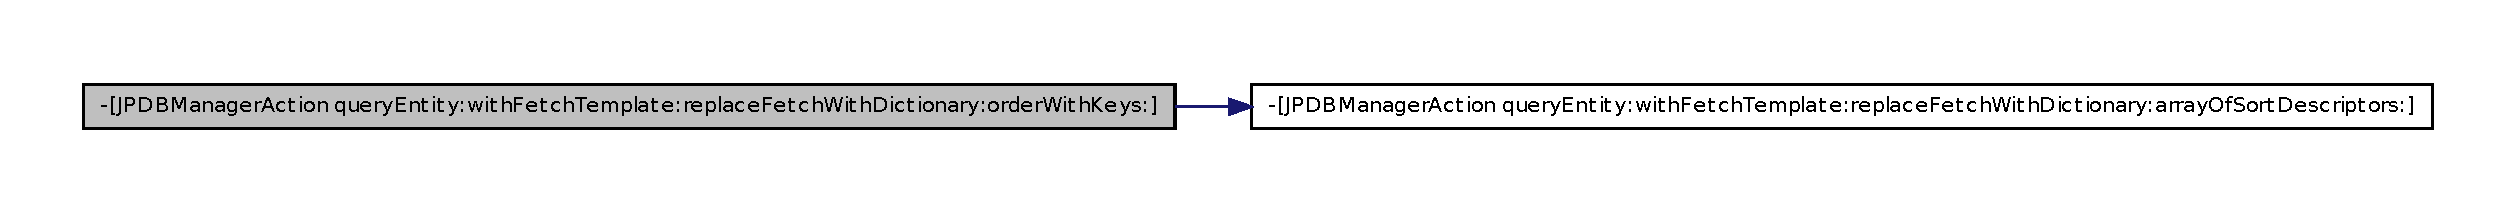
\includegraphics[width=400pt]{interface_j_p_d_b_manager_action_ac04b76b32d39ae9b412f99b3ac620a86_cgraph}
\end{center}
\end{figure}




Here is the caller graph for this function:
\nopagebreak
\begin{figure}[H]
\begin{center}
\leavevmode
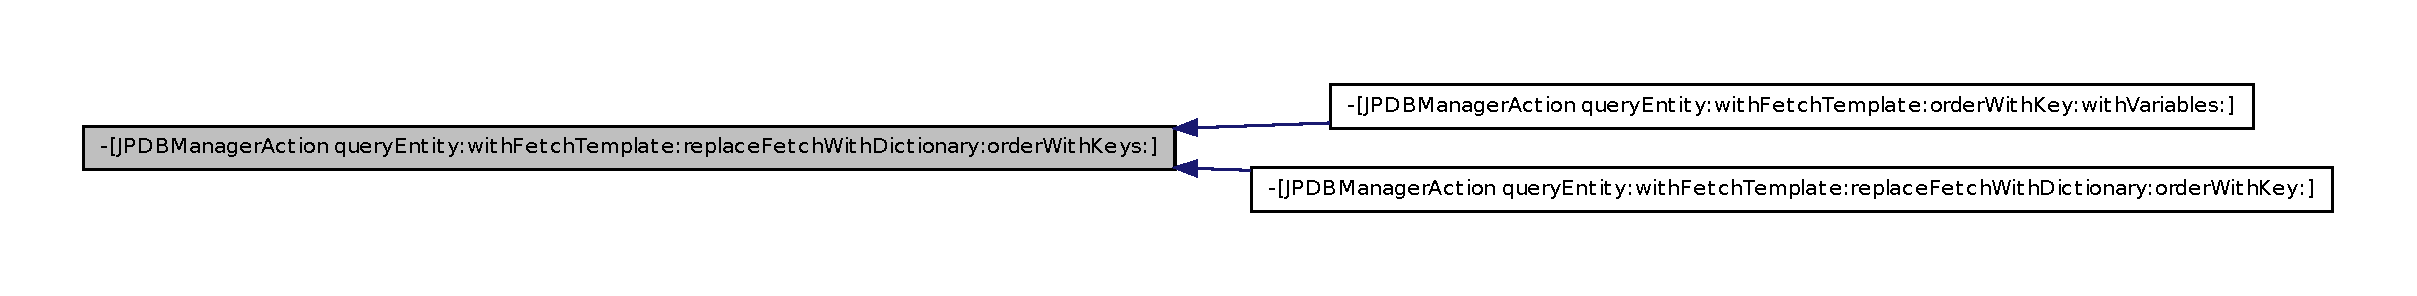
\includegraphics[width=400pt]{interface_j_p_d_b_manager_action_ac04b76b32d39ae9b412f99b3ac620a86_icgraph}
\end{center}
\end{figure}


\hypertarget{interface_j_p_d_b_manager_action_ad9f87e94c40f183732a44fd181ec96f6}{
\index{JPDBManagerAction@{JPDBManagerAction}!queryEntity:withFetchTemplate:replaceFetchWithDictionary:arrayOfSortDescriptors:@{queryEntity:withFetchTemplate:replaceFetchWithDictionary:arrayOfSortDescriptors:}}
\index{queryEntity:withFetchTemplate:replaceFetchWithDictionary:arrayOfSortDescriptors:@{queryEntity:withFetchTemplate:replaceFetchWithDictionary:arrayOfSortDescriptors:}!JPDBManagerAction@{JPDBManagerAction}}
\subsubsection[{queryEntity:withFetchTemplate:replaceFetchWithDictionary:arrayOfSortDescriptors:}]{\setlength{\rightskip}{0pt plus 5cm}-\/ (id) queryEntity: 
\begin{DoxyParamCaption}
\item[{dummy(NSString$\ast$)}]{anEntityName}
\item[{withFetchTemplate:(NSString$\ast$)}]{anFetchName}
\item[{replaceFetchWithDictionary:(NSDictionary$\ast$)}]{variablesListAndValues}
\item[{arrayOfSortDescriptors:(NSArray$\ast$)}]{anArrayOfSortDescriptors}
\end{DoxyParamCaption}
}}
\label{interface_j_p_d_b_manager_action_ad9f87e94c40f183732a44fd181ec96f6}


Query specified Entity using one specified Fetch Template name. 


\begin{DoxyParams}{Parameters}
{\em anEntityName} & The Entity Name. \\
\hline
{\em anFetchName} & An Fetch Template to perform the query. \\
\hline
{\em variablesListAndValues} & An Dictionary with Keys and Values to replace on the pre formatted Fetch Template. \\
\hline
{\em anArrayOfSortDescriptors} & An Array of Key attributes to sort the result. \\
\hline
\end{DoxyParams}
\begin{DoxyReturn}{Returns}
One unordered collection with queried data Objects. The Class of this collection is setted by \#returnQueryAsArray property. 
\end{DoxyReturn}


Here is the caller graph for this function:
\nopagebreak
\begin{figure}[H]
\begin{center}
\leavevmode
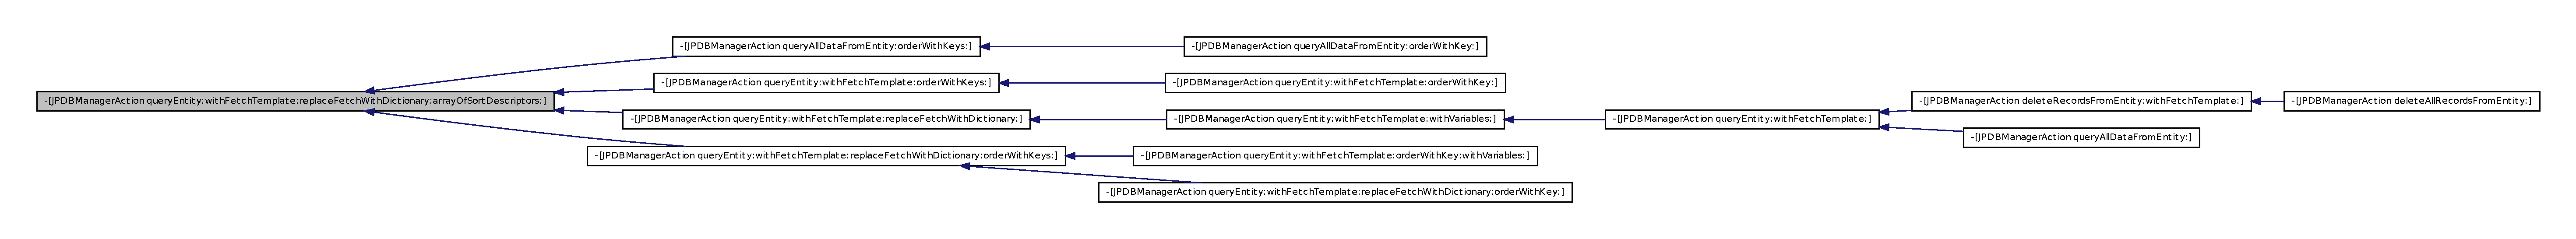
\includegraphics[width=400pt]{interface_j_p_d_b_manager_action_ad9f87e94c40f183732a44fd181ec96f6_icgraph}
\end{center}
\end{figure}


\hypertarget{interface_j_p_d_b_manager_action_a0b4bbc0a957856f7e0166d58f987e8dc}{
\index{JPDBManagerAction@{JPDBManagerAction}!queryEntity:withPredicate:@{queryEntity:withPredicate:}}
\index{queryEntity:withPredicate:@{queryEntity:withPredicate:}!JPDBManagerAction@{JPDBManagerAction}}
\subsubsection[{queryEntity:withPredicate:}]{\setlength{\rightskip}{0pt plus 5cm}-\/ (id) queryEntity: 
\begin{DoxyParamCaption}
\item[{dummy(NSString$\ast$)}]{anEntityName}
\item[{withPredicate:(NSPredicate$\ast$)}]{anPredicate}
\end{DoxyParamCaption}
}}
\label{interface_j_p_d_b_manager_action_a0b4bbc0a957856f7e0166d58f987e8dc}


Query specified Entity using one custom NSPredicate Object. 


\begin{DoxyParams}{Parameters}
{\em anEntityName} & The Entity Name. @ \\
\hline
{\em anPredicate} & An {\bfseries NSPredicate} object defining the query. \\
\hline
\end{DoxyParams}
\begin{DoxyReturn}{Returns}
One unordered collection with queried data Objects. The Class of this collection is setted by \#returnQueryAsArray property. 
\end{DoxyReturn}


Here is the call graph for this function:
\nopagebreak
\begin{figure}[H]
\begin{center}
\leavevmode
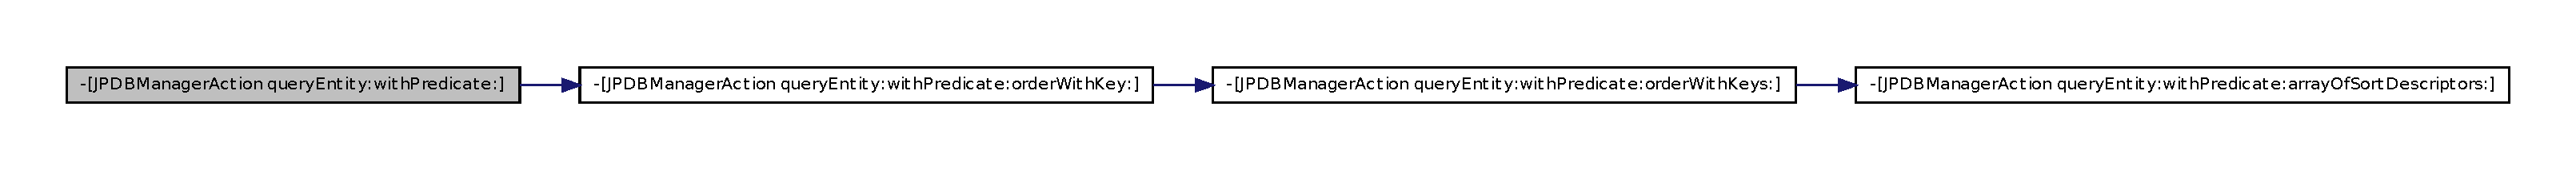
\includegraphics[width=400pt]{interface_j_p_d_b_manager_action_a0b4bbc0a957856f7e0166d58f987e8dc_cgraph}
\end{center}
\end{figure}


\hypertarget{interface_j_p_d_b_manager_action_a59b25a33e515e04dbf7e7d83855e86d1}{
\index{JPDBManagerAction@{JPDBManagerAction}!queryEntity:withPredicate:orderWithKey:@{queryEntity:withPredicate:orderWithKey:}}
\index{queryEntity:withPredicate:orderWithKey:@{queryEntity:withPredicate:orderWithKey:}!JPDBManagerAction@{JPDBManagerAction}}
\subsubsection[{queryEntity:withPredicate:orderWithKey:}]{\setlength{\rightskip}{0pt plus 5cm}-\/ (id) queryEntity: 
\begin{DoxyParamCaption}
\item[{dummy(NSString$\ast$)}]{anEntityName}
\item[{withPredicate:(NSPredicate$\ast$)}]{anPredicate}
\item[{orderWithKey:(id)}]{anKey}
\end{DoxyParamCaption}
}}
\label{interface_j_p_d_b_manager_action_a59b25a33e515e04dbf7e7d83855e86d1}


Query specified Entity using one custom NSPredicate Object. 


\begin{DoxyParams}{Parameters}
{\em anEntityName} & The Entity Name. \\
\hline
{\em anPredicate} & An {\bfseries NSPredicate} object defining the query. \\
\hline
{\em anKey} & One Key attribute to sort the result. \\
\hline
\end{DoxyParams}
\begin{DoxyReturn}{Returns}
One unordered collection with queried data Objects. The Class of this collection is setted by \#returnQueryAsArray property. 
\end{DoxyReturn}


Here is the call graph for this function:
\nopagebreak
\begin{figure}[H]
\begin{center}
\leavevmode
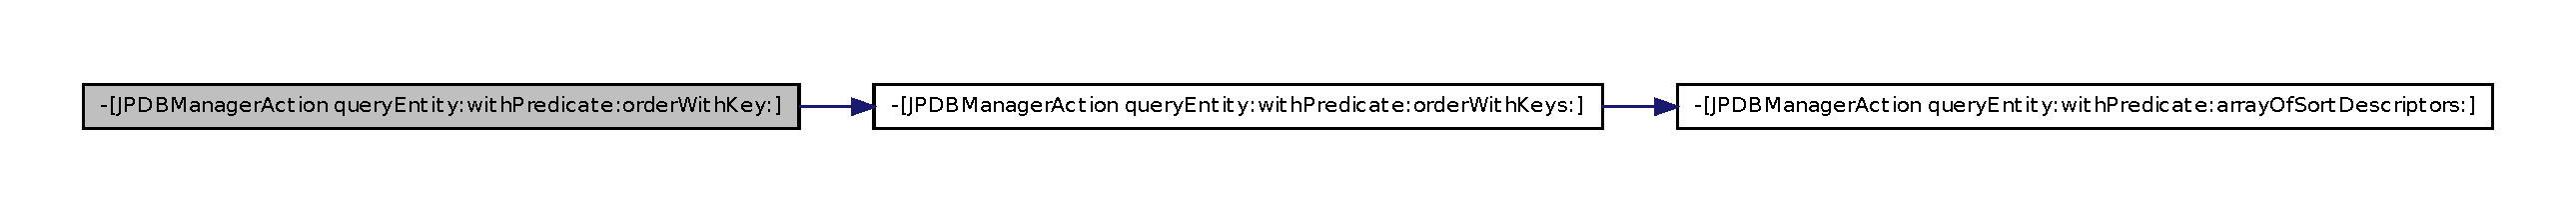
\includegraphics[width=400pt]{interface_j_p_d_b_manager_action_a59b25a33e515e04dbf7e7d83855e86d1_cgraph}
\end{center}
\end{figure}




Here is the caller graph for this function:
\nopagebreak
\begin{figure}[H]
\begin{center}
\leavevmode
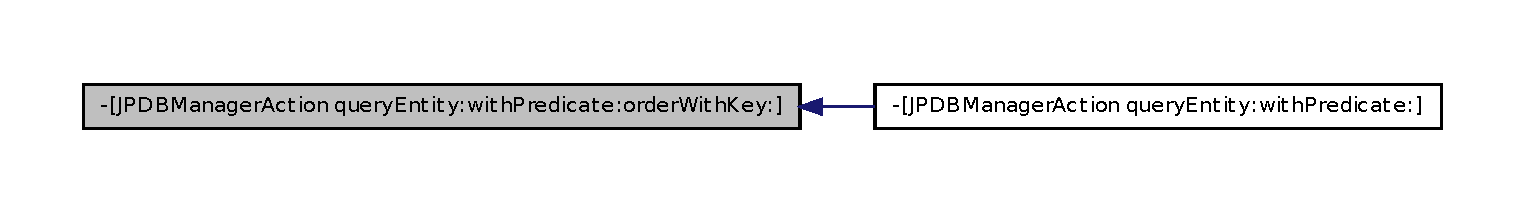
\includegraphics[width=400pt]{interface_j_p_d_b_manager_action_a59b25a33e515e04dbf7e7d83855e86d1_icgraph}
\end{center}
\end{figure}


\hypertarget{interface_j_p_d_b_manager_action_a8b9de476586b7352658c07c6f9b92bd9}{
\index{JPDBManagerAction@{JPDBManagerAction}!queryEntity:withPredicate:orderWithKeys:@{queryEntity:withPredicate:orderWithKeys:}}
\index{queryEntity:withPredicate:orderWithKeys:@{queryEntity:withPredicate:orderWithKeys:}!JPDBManagerAction@{JPDBManagerAction}}
\subsubsection[{queryEntity:withPredicate:orderWithKeys:}]{\setlength{\rightskip}{0pt plus 5cm}-\/ (id) queryEntity: 
\begin{DoxyParamCaption}
\item[{dummy(NSString$\ast$)}]{anEntityName}
\item[{withPredicate:(NSPredicate$\ast$)}]{anPredicate}
\item[{orderWithKeys:(id)}]{listOfKeys}
\item[{,}]{NS\_\-REQUIRES\_\-NIL\_\-TERMINATION}
\end{DoxyParamCaption}
}}
\label{interface_j_p_d_b_manager_action_a8b9de476586b7352658c07c6f9b92bd9}


Query specified Entity using one custom NSPredicate Object. 


\begin{DoxyParams}{Parameters}
{\em anEntityName} & The Entity Name. \\
\hline
{\em anPredicate} & An {\bfseries NSPredicate} object defining the query. \\
\hline
{\em listOfKeys} & Accept one or more Key Attributes to sort the result. Doesn't forget to terminate the list with an 'nil' token. \\
\hline
\end{DoxyParams}
\begin{DoxyReturn}{Returns}
One unordered collection with queried data Objects. The Class of this collection is setted by \#returnQueryAsArray property. 
\end{DoxyReturn}


Here is the call graph for this function:
\nopagebreak
\begin{figure}[H]
\begin{center}
\leavevmode
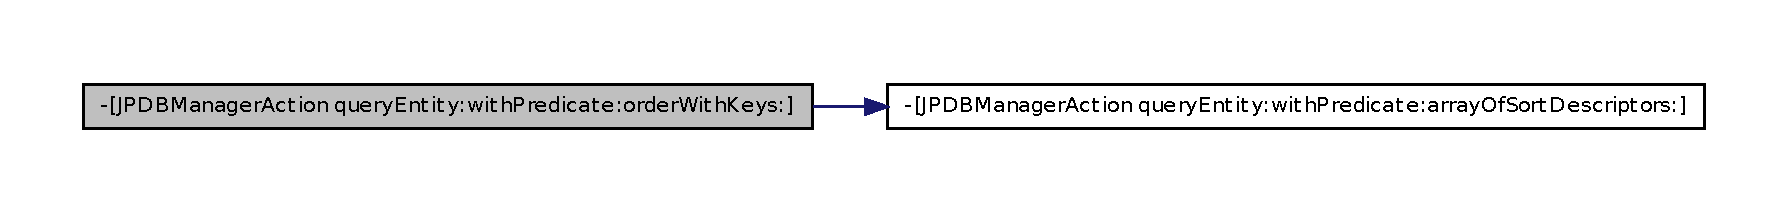
\includegraphics[width=400pt]{interface_j_p_d_b_manager_action_a8b9de476586b7352658c07c6f9b92bd9_cgraph}
\end{center}
\end{figure}




Here is the caller graph for this function:
\nopagebreak
\begin{figure}[H]
\begin{center}
\leavevmode
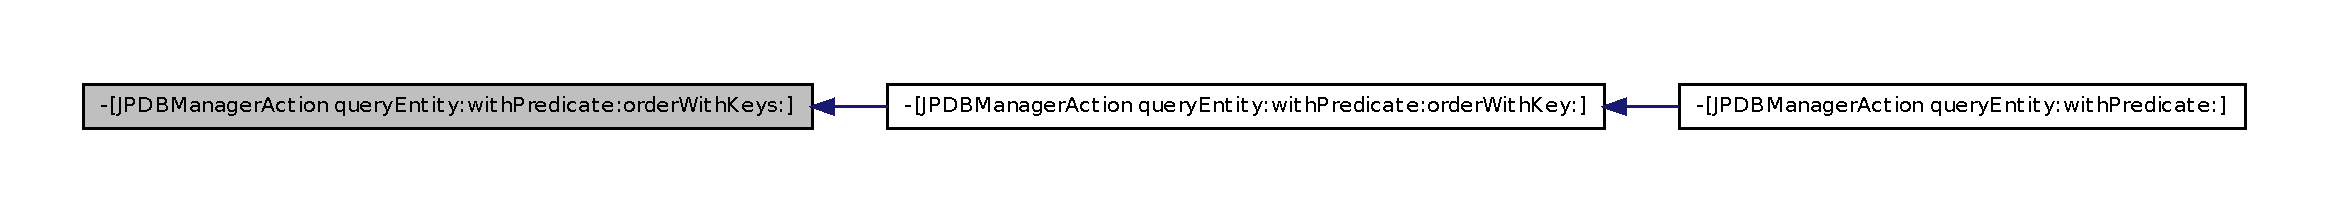
\includegraphics[width=400pt]{interface_j_p_d_b_manager_action_a8b9de476586b7352658c07c6f9b92bd9_icgraph}
\end{center}
\end{figure}


\hypertarget{interface_j_p_d_b_manager_action_aa7020d4c7938f259bab678b4c9b0a056}{
\index{JPDBManagerAction@{JPDBManagerAction}!queryEntity:withPredicate:arrayOfSortDescriptors:@{queryEntity:withPredicate:arrayOfSortDescriptors:}}
\index{queryEntity:withPredicate:arrayOfSortDescriptors:@{queryEntity:withPredicate:arrayOfSortDescriptors:}!JPDBManagerAction@{JPDBManagerAction}}
\subsubsection[{queryEntity:withPredicate:arrayOfSortDescriptors:}]{\setlength{\rightskip}{0pt plus 5cm}-\/ (id) queryEntity: 
\begin{DoxyParamCaption}
\item[{dummy(NSString$\ast$)}]{anEntityName}
\item[{withPredicate:(NSPredicate$\ast$)}]{anPredicate}
\item[{arrayOfSortDescriptors:(NSArray$\ast$)}]{anArrayOfSortDescriptors}
\end{DoxyParamCaption}
}}
\label{interface_j_p_d_b_manager_action_aa7020d4c7938f259bab678b4c9b0a056}


Query specified Entity using one custom NSPredicate Object. 


\begin{DoxyParams}{Parameters}
{\em anEntityName} & The Entity Name. \\
\hline
{\em anPredicate} & An {\bfseries NSPredicate} object defining the query. \\
\hline
{\em anArrayOfSortDescriptors} & An Array of Key attributes to sort the result. \\
\hline
\end{DoxyParams}
\begin{DoxyReturn}{Returns}
One unordered collection with queried data Objects. The Class of this collection is setted by \#returnQueryAsArray property. 
\end{DoxyReturn}


Here is the caller graph for this function:
\nopagebreak
\begin{figure}[H]
\begin{center}
\leavevmode
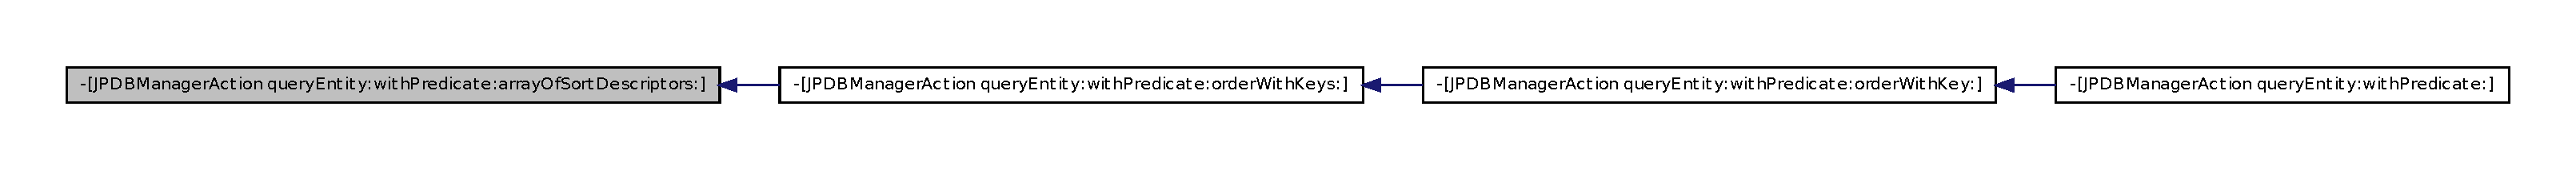
\includegraphics[width=400pt]{interface_j_p_d_b_manager_action_aa7020d4c7938f259bab678b4c9b0a056_icgraph}
\end{center}
\end{figure}


\hypertarget{interface_j_p_d_b_manager_action_ac566a65fcbfa1026f42954648d60e6b8}{
\index{JPDBManagerAction@{JPDBManagerAction}!deleteRecord:@{deleteRecord:}}
\index{deleteRecord:@{deleteRecord:}!JPDBManagerAction@{JPDBManagerAction}}
\subsubsection[{deleteRecord:}]{\setlength{\rightskip}{0pt plus 5cm}-\/ (void) deleteRecord: 
\begin{DoxyParamCaption}
\item[{dummy(id)}]{anObject}
\end{DoxyParamCaption}
}}
\label{interface_j_p_d_b_manager_action_ac566a65fcbfa1026f42954648d60e6b8}


Delete specified Record from his Entity on the Database. 

This method will use the \hyperlink{interface_j_p_d_b_manager_action_ad0060c13ad4e89eb23c60ad123250505}{commitTransaction} property to decide if commit automatically this change. 
\begin{DoxyParams}{Parameters}
{\em anObject} & Record object to delete. \\
\hline
\end{DoxyParams}


Here is the call graph for this function:
\nopagebreak
\begin{figure}[H]
\begin{center}
\leavevmode
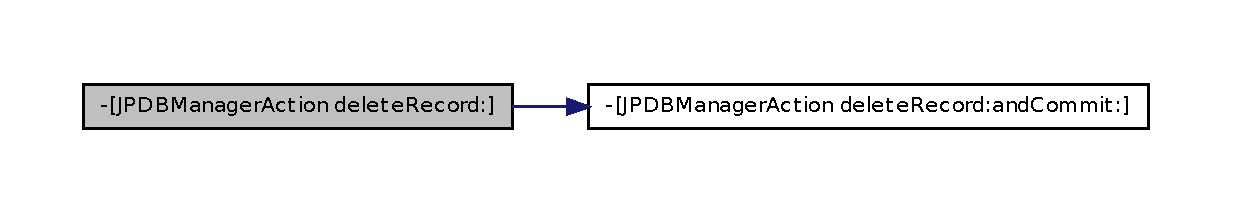
\includegraphics[width=400pt]{interface_j_p_d_b_manager_action_ac566a65fcbfa1026f42954648d60e6b8_cgraph}
\end{center}
\end{figure}


\hypertarget{interface_j_p_d_b_manager_action_a7a8d41ed1791761c1996af5d031e41a7}{
\index{JPDBManagerAction@{JPDBManagerAction}!deleteRecord:andCommit:@{deleteRecord:andCommit:}}
\index{deleteRecord:andCommit:@{deleteRecord:andCommit:}!JPDBManagerAction@{JPDBManagerAction}}
\subsubsection[{deleteRecord:andCommit:}]{\setlength{\rightskip}{0pt plus 5cm}-\/ (void) deleteRecord: 
\begin{DoxyParamCaption}
\item[{dummy(id)}]{anObject}
\item[{andCommit:(BOOL)}]{commit}
\end{DoxyParamCaption}
}}
\label{interface_j_p_d_b_manager_action_a7a8d41ed1791761c1996af5d031e41a7}


Delete specified Record from his Entity on the Database. 


\begin{DoxyParams}{Parameters}
{\em anObject} & Record object to delete. \\
\hline
{\em commit} & Specify if you want to commit or not this operation immediattelly. \\
\hline
\end{DoxyParams}


Here is the caller graph for this function:
\nopagebreak
\begin{figure}[H]
\begin{center}
\leavevmode
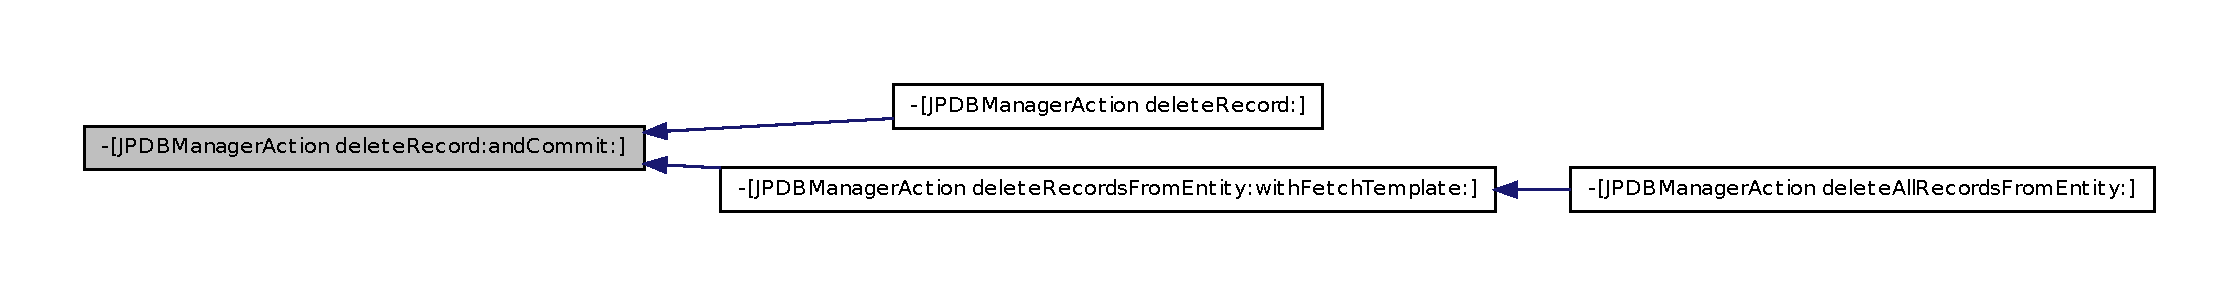
\includegraphics[width=400pt]{interface_j_p_d_b_manager_action_a7a8d41ed1791761c1996af5d031e41a7_icgraph}
\end{center}
\end{figure}


\hypertarget{interface_j_p_d_b_manager_action_af85b28a738631615ad0e4030500ce71a}{
\index{JPDBManagerAction@{JPDBManagerAction}!deleteRecordsFromEntity:withFetchTemplate:@{deleteRecordsFromEntity:withFetchTemplate:}}
\index{deleteRecordsFromEntity:withFetchTemplate:@{deleteRecordsFromEntity:withFetchTemplate:}!JPDBManagerAction@{JPDBManagerAction}}
\subsubsection[{deleteRecordsFromEntity:withFetchTemplate:}]{\setlength{\rightskip}{0pt plus 5cm}-\/ (void) deleteRecordsFromEntity: 
\begin{DoxyParamCaption}
\item[{dummy(NSString$\ast$)}]{anEntityName}
\item[{withFetchTemplate:(NSString$\ast$)}]{anFetchName}
\end{DoxyParamCaption}
}}
\label{interface_j_p_d_b_manager_action_af85b28a738631615ad0e4030500ce71a}


Delete all records queried by the specified Fetch Template. 

This method will use the \hyperlink{interface_j_p_d_b_manager_action_ad0060c13ad4e89eb23c60ad123250505}{commitTransaction} property to decide if commit automatically this change. 
\begin{DoxyParams}{Parameters}
{\em anEntityName} & The Entity Name. \\
\hline
{\em anFetchName} & An Fetch Template to perform the query. \\
\hline
\end{DoxyParams}


Here is the call graph for this function:
\nopagebreak
\begin{figure}[H]
\begin{center}
\leavevmode
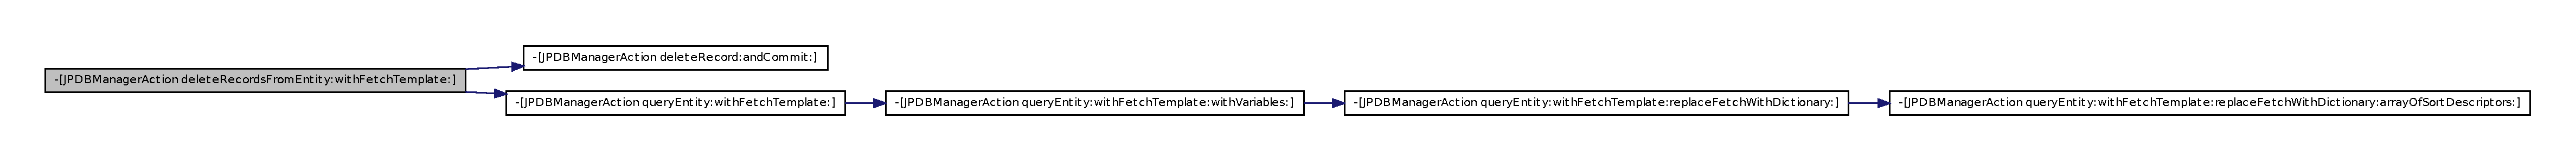
\includegraphics[width=400pt]{interface_j_p_d_b_manager_action_af85b28a738631615ad0e4030500ce71a_cgraph}
\end{center}
\end{figure}




Here is the caller graph for this function:
\nopagebreak
\begin{figure}[H]
\begin{center}
\leavevmode
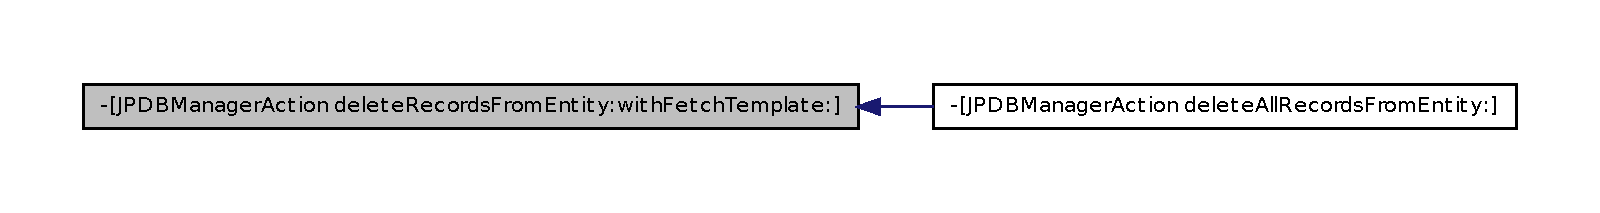
\includegraphics[width=400pt]{interface_j_p_d_b_manager_action_af85b28a738631615ad0e4030500ce71a_icgraph}
\end{center}
\end{figure}


\hypertarget{interface_j_p_d_b_manager_action_a1a7a137d9a6617366523dca5a59174a0}{
\index{JPDBManagerAction@{JPDBManagerAction}!deleteAllRecordsFromEntity:@{deleteAllRecordsFromEntity:}}
\index{deleteAllRecordsFromEntity:@{deleteAllRecordsFromEntity:}!JPDBManagerAction@{JPDBManagerAction}}
\subsubsection[{deleteAllRecordsFromEntity:}]{\setlength{\rightskip}{0pt plus 5cm}-\/ (void) deleteAllRecordsFromEntity: 
\begin{DoxyParamCaption}
\item[{dummy(NSString$\ast$)}]{anEntityName}
\end{DoxyParamCaption}
}}
\label{interface_j_p_d_b_manager_action_a1a7a137d9a6617366523dca5a59174a0}


Delete all Records from specified Entity. 

This could be a consuming operation on large databases. 
\begin{DoxyParams}{Parameters}
{\em anEntityName} & The Entity Name. \\
\hline
\end{DoxyParams}


Here is the call graph for this function:
\nopagebreak
\begin{figure}[H]
\begin{center}
\leavevmode
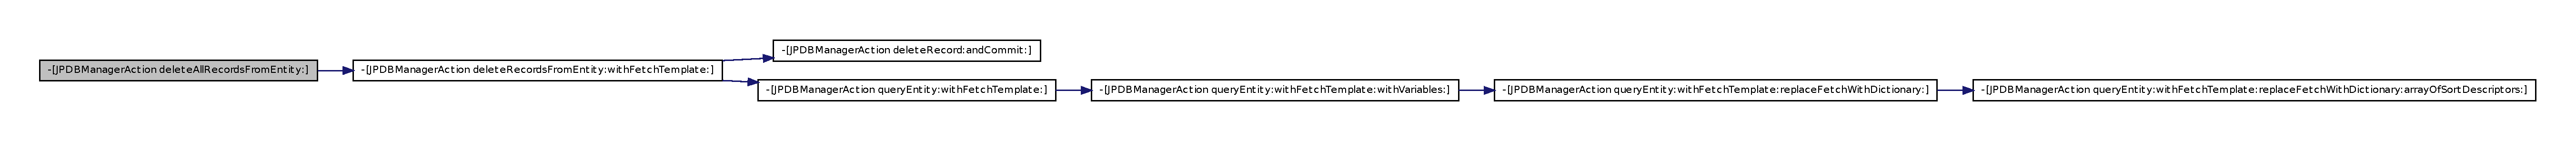
\includegraphics[width=400pt]{interface_j_p_d_b_manager_action_a1a7a137d9a6617366523dca5a59174a0_cgraph}
\end{center}
\end{figure}


\hypertarget{interface_j_p_d_b_manager_action_a64efbdc0e61408df85b45629141871e6}{
\index{JPDBManagerAction@{JPDBManagerAction}!createNewRecordForEntity:@{createNewRecordForEntity:}}
\index{createNewRecordForEntity:@{createNewRecordForEntity:}!JPDBManagerAction@{JPDBManagerAction}}
\subsubsection[{createNewRecordForEntity:}]{\setlength{\rightskip}{0pt plus 5cm}-\/ (id) createNewRecordForEntity: 
\begin{DoxyParamCaption}
\item[{dummy(NSString$\ast$)}]{anEntityName}
\end{DoxyParamCaption}
}}
\label{interface_j_p_d_b_manager_action_a64efbdc0e61408df85b45629141871e6}


Create and return a new record for specified Entity. 


\begin{DoxyParams}{Parameters}
{\em anEntityName} & The Entity Name. \\
\hline
\end{DoxyParams}
\begin{DoxyReturn}{Returns}
New empty Record. 
\end{DoxyReturn}


Here is the call graph for this function:
\nopagebreak
\begin{figure}[H]
\begin{center}
\leavevmode
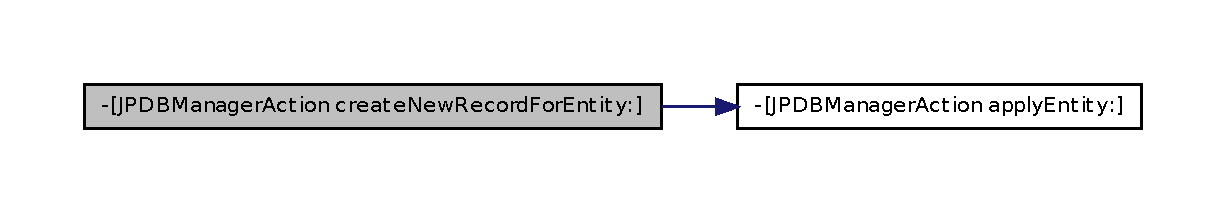
\includegraphics[width=400pt]{interface_j_p_d_b_manager_action_a64efbdc0e61408df85b45629141871e6_cgraph}
\end{center}
\end{figure}




\subsection{Property Documentation}
\hypertarget{interface_j_p_d_b_manager_action_ad0060c13ad4e89eb23c60ad123250505}{
\index{JPDBManagerAction@{JPDBManagerAction}!commitTransaction@{commitTransaction}}
\index{commitTransaction@{commitTransaction}!JPDBManagerAction@{JPDBManagerAction}}
\subsubsection[{commitTransaction}]{\setlength{\rightskip}{0pt plus 5cm}-\/ (BOOL) commitTransaction\hspace{0.3cm}{\ttfamily  \mbox{[}read, write, assign\mbox{]}}}}
\label{interface_j_p_d_b_manager_action_ad0060c13ad4e89eb23c60ad123250505}


Set if the Manager should commit this transaction immediatelly or not. 

\par
 Default value is {\bfseries NO}. \hypertarget{interface_j_p_d_b_manager_action_ae603fd48edaea29a115b90a19f440ab8}{
\index{JPDBManagerAction@{JPDBManagerAction}!returnObjectsAsFault@{returnObjectsAsFault}}
\index{returnObjectsAsFault@{returnObjectsAsFault}!JPDBManagerAction@{JPDBManagerAction}}
\subsubsection[{returnObjectsAsFault}]{\setlength{\rightskip}{0pt plus 5cm}-\/ (BOOL) returnObjectsAsFault\hspace{0.3cm}{\ttfamily  \mbox{[}read, write, assign\mbox{]}}}}
\label{interface_j_p_d_b_manager_action_ae603fd48edaea29a115b90a19f440ab8}


Define if the Result objects of some query should be as Core Data Fault. 

Default value is {\bfseries NO}. \hypertarget{interface_j_p_d_b_manager_action_a0e153817018f1c41c7fa6bd5780ef09a}{
\index{JPDBManagerAction@{JPDBManagerAction}!ascendingOrder@{ascendingOrder}}
\index{ascendingOrder@{ascendingOrder}!JPDBManagerAction@{JPDBManagerAction}}
\subsubsection[{ascendingOrder}]{\setlength{\rightskip}{0pt plus 5cm}-\/ (BOOL) ascendingOrder\hspace{0.3cm}{\ttfamily  \mbox{[}read, write, assign\mbox{]}}}}
\label{interface_j_p_d_b_manager_action_a0e153817018f1c41c7fa6bd5780ef09a}


Define if the order of the results of some query should be Ascending or Descending. 

Note that by performance you should set this value before apply any Key sort attribute. You can do it after, but the manager will recreate every sort key again. Default value is {\bfseries YES}. \hypertarget{interface_j_p_d_b_manager_action_aecdffb5193789cbd3e4704e71c90972c}{
\index{JPDBManagerAction@{JPDBManagerAction}!returnActionAsArray@{returnActionAsArray}}
\index{returnActionAsArray@{returnActionAsArray}!JPDBManagerAction@{JPDBManagerAction}}
\subsubsection[{returnActionAsArray}]{\setlength{\rightskip}{0pt plus 5cm}-\/ (BOOL) returnActionAsArray\hspace{0.3cm}{\ttfamily  \mbox{[}read, write, assign\mbox{]}}}}
\label{interface_j_p_d_b_manager_action_aecdffb5193789cbd3e4704e71c90972c}


Set if the Result of this action should be an {\bfseries NSArray} or an {\bfseries NSFetchedResultsController} object. 

\par
 Default value is {\bfseries YES}. \hypertarget{interface_j_p_d_b_manager_action_ad679e0229dbddd7d5c87a6348d33fc9e}{
\index{JPDBManagerAction@{JPDBManagerAction}!startFetchInLine@{startFetchInLine}}
\index{startFetchInLine@{startFetchInLine}!JPDBManagerAction@{JPDBManagerAction}}
\subsubsection[{startFetchInLine}]{\setlength{\rightskip}{0pt plus 5cm}-\/ (int) startFetchInLine\hspace{0.3cm}{\ttfamily  \mbox{[}read, write, assign\mbox{]}}}}
\label{interface_j_p_d_b_manager_action_ad679e0229dbddd7d5c87a6348d33fc9e}


Set the initial row result to return from Query Methods results. 

Combine this set with the \hyperlink{interface_j_p_d_b_manager_action_a768d19efb483654b753bdc3a8bf1a197}{limitFetchResults} property.\par
 Default value is {\bfseries 0}. \hypertarget{interface_j_p_d_b_manager_action_a768d19efb483654b753bdc3a8bf1a197}{
\index{JPDBManagerAction@{JPDBManagerAction}!limitFetchResults@{limitFetchResults}}
\index{limitFetchResults@{limitFetchResults}!JPDBManagerAction@{JPDBManagerAction}}
\subsubsection[{limitFetchResults}]{\setlength{\rightskip}{0pt plus 5cm}-\/ (int) limitFetchResults\hspace{0.3cm}{\ttfamily  \mbox{[}read, write, assign\mbox{]}}}}
\label{interface_j_p_d_b_manager_action_a768d19efb483654b753bdc3a8bf1a197}


Set the maximum rows to return from Query Methods results. 

Combine this set with the \hyperlink{interface_j_p_d_b_manager_action_ad679e0229dbddd7d5c87a6348d33fc9e}{startFetchInLine} property.\par
 Default value is {\bfseries 0}, it means that all rows in the Entity will be retrieved. 

The documentation for this class was generated from the following files:\begin{DoxyCompactItemize}
\item 
/Users/Paulo/Projects/JUMP/JUMPDatabase/Headers/JPDBManagerAction.h\item 
/Users/Paulo/Projects/JUMP/JUMPDatabase/Sources/JPDBManagerAction.m\end{DoxyCompactItemize}

\hypertarget{interface_j_p_d_b_manager_singleton}{
\section{JPDBManagerSingleton Class Reference}
\label{interface_j_p_d_b_manager_singleton}\index{JPDBManagerSingleton@{JPDBManagerSingleton}}
}


Singleton instance of \hyperlink{interface_j_p_d_b_manager}{Database Manager} that handle the {\bfseries Core Data Environment}.  




{\ttfamily \#import $<$JPDBManagerSingleton.h$>$}



Inheritance diagram for JPDBManagerSingleton:
\nopagebreak
\begin{figure}[H]
\begin{center}
\leavevmode
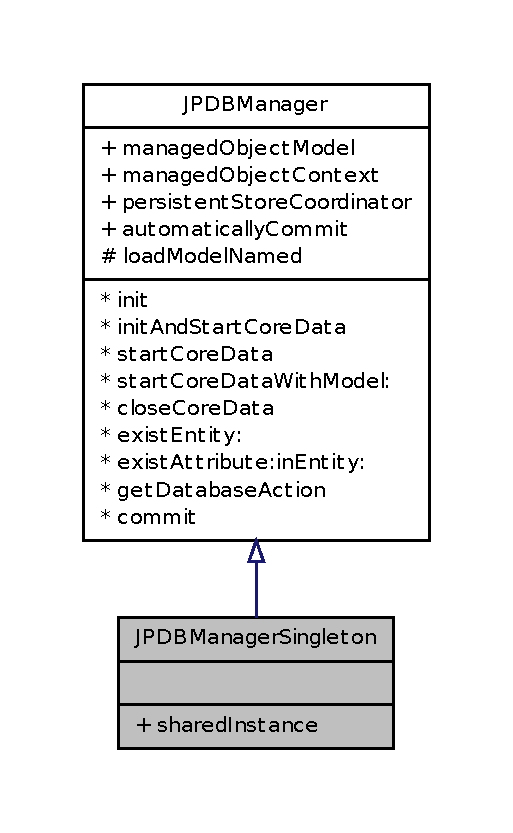
\includegraphics[width=246pt]{interface_j_p_d_b_manager_singleton__inherit__graph}
\end{center}
\end{figure}


Collaboration diagram for JPDBManagerSingleton:
\nopagebreak
\begin{figure}[H]
\begin{center}
\leavevmode
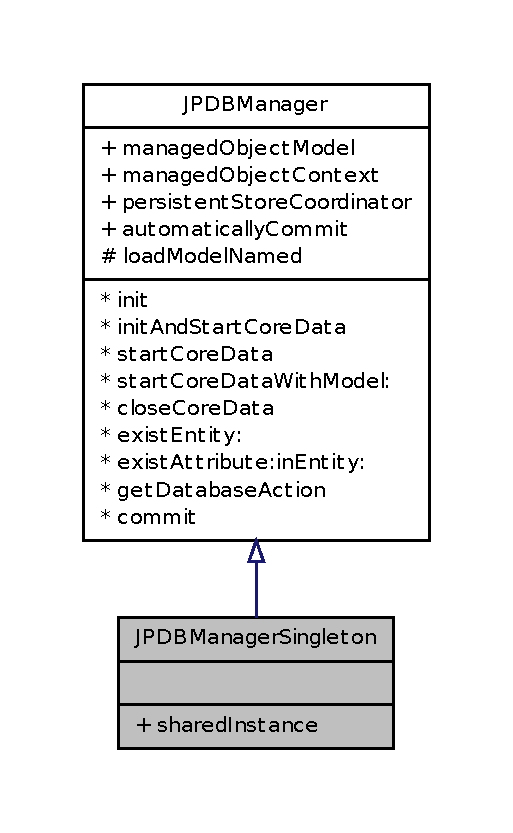
\includegraphics[width=246pt]{interface_j_p_d_b_manager_singleton__coll__graph}
\end{center}
\end{figure}
\subsection*{Static Public Member Functions}
\begin{DoxyCompactItemize}
\item 
(\hyperlink{interface_j_p_d_b_manager_singleton}{JPDBManagerSingleton} $\ast$) + \hyperlink{interface_j_p_d_b_manager_singleton_a505d4d641b1b0adc616c6aba8c11951c}{sharedInstance}
\begin{DoxyCompactList}\small\item\em Init Singleton Class Instance. \item\end{DoxyCompactList}\end{DoxyCompactItemize}


\subsection{Detailed Description}
Singleton instance of \hyperlink{interface_j_p_d_b_manager}{Database Manager} that handle the {\bfseries Core Data Environment}. Note that you should initiate this class using the \hyperlink{interface_j_p_d_b_manager_singleton_a505d4d641b1b0adc616c6aba8c11951c}{sharedInstance (JPDBManagerSingleton)} method, if you try to initate using some of the \hyperlink{interface_j_p_d_b_manager}{JPDBManager} init methods an \hyperlink{errors_JPDBInvalidInitiator}{JPDBInvalidInitiator} exception will be raised. See \hyperlink{errors}{Handling Errors} for more informations.\par
 \par
 See the \hyperlink{basic_uses}{Basic Uses} to learn the basic concepts about this class. Also consult \hyperlink{errors}{Handling Errors} and \hyperlink{queries}{Performing Queries}.  

\subsection{Member Function Documentation}
\hypertarget{interface_j_p_d_b_manager_singleton_a505d4d641b1b0adc616c6aba8c11951c}{
\index{JPDBManagerSingleton@{JPDBManagerSingleton}!sharedInstance@{sharedInstance}}
\index{sharedInstance@{sharedInstance}!JPDBManagerSingleton@{JPDBManagerSingleton}}
\subsubsection[{sharedInstance}]{\setlength{\rightskip}{0pt plus 5cm}+ ({\bf JPDBManagerSingleton}$\ast$) sharedInstance 
\begin{DoxyParamCaption}
{}
\end{DoxyParamCaption}
}}
\label{interface_j_p_d_b_manager_singleton_a505d4d641b1b0adc616c6aba8c11951c}


Init Singleton Class Instance. 

This Method Initialize this class and/or return one singleton instance of it. 

The documentation for this class was generated from the following file:\begin{DoxyCompactItemize}
\item 
/Users/Paulo/Projects/JUMP/JUMPDatabase/Headers/JPDBManagerSingleton.h\end{DoxyCompactItemize}

\printindex
\end{document}
